\chapter{Stellar mass as a cluster mass proxy}\label{chp:proxy}

\begin{flushright}
  {\em ``It is the unknown we fear when we look upon death and darkness, nothing more.'' }\\

\ \

\normalsize
{J.~K.~Rowling -- Harry Potter and the Half-Blood Prince}  
\end{flushright}


\noindent{\emph{The work described in this chapter is part of {\bf Palmese et al., 2018} ``Stellar mass as a galaxy cluster mass proxy and stellar--to--halo connection in the Dark Energy Survey redMaPPer clusters'', currently in the DES collaboration review process, and the companion papers {\bf Welch, Annis, Lin, Palmese, Soares--Santos et al., in prep.,} and {\bf Pereira, Soares-Santos, Makler,  Annis, Lin, Palmese et al., 2018, MNRAS 474, 1361P}. }}

\section{Introduction}
Galaxy  clusters  are fundamental cosmological probes for large galaxy surveys such as the Dark Energy Survey.  The estimation of cosmological parameters from clusters abundance is allowed by the dependence of the halo mass function on cosmology (\citealt{press}; \citealt{sheth}; \citealt{tinker}), but this requires estimates of cluster total masses from the observables of our galaxy survey. In practice, we seek cluster mass observables (or mass proxies) that tightly correlate with halo mass. In other words they exhibit a low scatter in halo mass at fixed mass proxy (and vice versa).

Several cluster finders are based on the cluster red-sequence (e.g. \citealt{koester}; \citealt{hao}; \citealt{oguri}; \citealt{redpaper}). Amongst those, redMaPPer (\citealt{redpaper}) has been extensively studied and its mass proxy, the richness $\lambda$, calibrated for large photometric surveys such as the Sloan Digital Sky Survey (SDSS) and the DES over the past decade (\citealt{rozo09}; \citealt{lambda}; \citealt{extrinsicscatter}; \citealt{redmappersv}).  The richness is defined as the sum over the membership probabilities of all galaxies within the projected radius $R_\lambda$. This radius was calibrated against X-ray luminosity measurements $L_X$ in order to minimise the scatter in $L_X-\lambda$. \citet{2012ApJ...746..178R} set this variable to $R_\lambda = 1.0(\lambda/100)^{0.2} ~{\rm Mpc}/h$. On the other hand, there exists broad evidence that the content of clusters includes a non--negligible fraction of bluer, star--forming galaxies that do not follow the red sequence colour--magnitude relation, in particular towards increasing redshift (\citealt{oemler}; \citealt{butcher1}; \citealt{butcher2}; \citealt{Donahue}). This effect is known as the Butcher--Oemler effect.
Whether the inclusion of the blue cloud can improve cluster mass estimates for cosmology is a matter of debate (e.g. \citealt{extrinsicscatter}) and depends on the survey characteristics. At higher redshifts, the blue fraction becomes significant (it can reach $\sim 30\%$ below redshift $\sim 0.3$; \citealt{zu2}) and the red sequence is not as distinguishable in colour--magnitude space as at lower redshift. In these regimes, the inclusion of the bluer members may play a significant role in cluster abundance studies of DES and other on-going and future photometric surveys (the Large Synoptic Sky Survey, Euclid) that push towards higher redshifts, $z=1$ and beyond. One clear advantage of including blue galaxies in cluster catalogs is in studying cluster properties and their evolution with redshift, in particular the Butcher--Oemler effect and quenching mechanisms. Moreover, cluster finders able to identify also cluster members that do not belong to the red sequence (\citealt{miller05}; \citealt{vt}) already exist. We are particularly interested in building a mass proxy to implement in the Voronoi--Tessellation (VT) cluster finder, developed by DES collaborators in \citet{vt}. The VT algorithm builds a 2--dimensionsional tessellation in photometric redshift shells and flags galaxies that lie in high density cells as cluster members. The density threshold is taken from estimates of the 2-point correlation function. The original mass proxy delivered by VT was $N_{VT}$, the number of members identified. In a work based on DES SV data (\citealt{2015MNRAS.454.2305S}), the scatter in the $N_{VT}$--mass relation was shown to be too large for any cosmological analysis. For these reasons, we develop a low--scatter mass proxy for cluster finders that are not red-sequence based.

Previous works (for example \citealt{andreon12}) have exploited stellar masses as a possible cluster mass proxy. We here extend this study by using a larger sample of X-ray clusters for calibration and by complementing the stellar mass estimates with a membership probability scheme. We call this mass proxy ``$\mu_\star$''. It is defined as the sum of the stellar mass of cluster galaxies weighted by their membership probability, as we will see in Eq. (\ref{eq:mustar}). A feasibility study for stellar mass computation with DES data has been presented in Chapter \ref{chp:rxj}, where we found that stellar masses of clusters members can be recovered within 25\% of HST-CLASH values. We therefore apply our method to a well-established cluster catalog, the DES Year 1 (Y1) redMaPPer catalog. Nevertheless, this mass proxy can easily be used with other, non-red-sequence based, cluster finders.\\

This Section is structured as follows. In Section \ref{datasec} we describe the DES Y1 galaxy catalog, the Y1 redMaPPer catalog  and the X-ray clusters catalog used. In Section \ref{methodsec} we describe the method used to compute cluster stellar masses, the completeness of the sample, and the membership probability assignment scheme. Finally in Sections \ref{calibsec} and \ref{wlcalib} we calibrate our mass proxy against X--ray and weak lensing measurements.

\section{Data}\label{datasec}

\subsection{DES Year 1and Year 3 data}
The data used in this Chapter come from the first year of observations (September 2013 -- February 2014, \citealt{y1}) and cover $1,839~ {\rm deg}^2$ with up to 4 passes per filter. At the time of writing, five observing seasons have been completed.

The median $10\sigma$ limiting magnitudes of Y1 data for galaxies are $g = 23.4$, $r = 23.2$, $i = 22.5$, $z = 21.8$, and $Y = 20.1$.
\citet{firstyear} made further selections to produce a high-quality object catalog called the Y1A1 ``gold'' catalog.

\begin{figure}\centering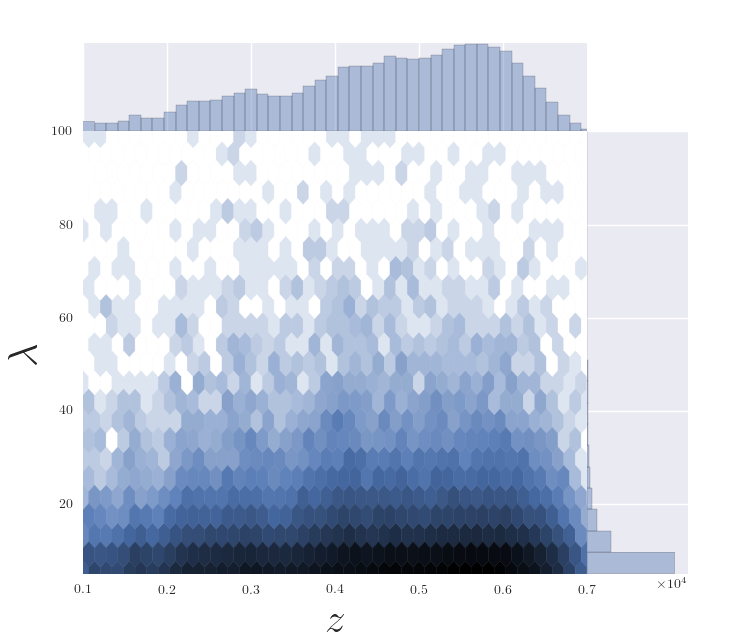
\includegraphics[width=0.7\textwidth]{./chapters/chapter5/figs/f2.png}\caption{Distribution in richness $\lambda$ and redshift for the volume--limited sample of DES Year 1 redMaPPer clusters used in this work.}\label{fig:clusters}\end{figure}

The cluster catalog used here is the cosmology Y1 redMaPPer catalog v6.4.17 with richness $\lambda>5$, which consists of more than $76,000$ clusters. The redshift estimate for each cluster is obtained by maximizing the probability that the observed color--distribution of likely members matches the self--calibrated red sequence model of redMaPPer. The cosmology catalog is built such that it is volume limited and therefore simplifies our analysis with respect to selection effects.
%we can ignore selection effects on our sample. 
The 2D distribution of richness and redshift of this sample is shown in Figure \ref{fig:clusters}. Note that the volume is defined locally, so that it will depend on depth and masking at different positions, thus the decrease at $z>0.6$. The centre position (given by the galaxy with the highest central probability $p_{cen}$) and the cluster redshift are the only outputs used from this catalog.
The galaxies associated with each cluster are taken from the Y1A1 gold catalog. We select objects with \texttt{MODEST\_CLASS}=1 in order to exclude sources that are likely not to be galaxies. 

While the cluster catalog is based on Y1 data, the photometry comes from the deeper Year 3 data. The Year 3 catalog contains $\sim 400$ million objects over $\sim 5,000~{\rm deg}^2$ (of which $\sim 310$ million are galaxies), and it has the following median $10\sigma$ coadded depths for a $1.95''$ diameter aperture: $g = 24.33$, $r = 24.08$, $i = 23.44$, $z = 22.69$, and $Y = 21.44$ mag (\citealt{dr1}). The photometry  is the result of the Multi-Object Fitting (MOF) pipeline that uses the \texttt{ngmix} code.\footnote{\url{https://github.com/esheldon/ngmix}}

In order to compute the membership probabilities (as described in Section \ref{tomustar}), we use photo-$z$s from the template-based Bayesian Photometric Redshifts (BPZ) algorithm (\citealt{bpz}). The catalog used in this work uses the same procedure as outlined in \cite{Hoyle}. Briefly, six basic templates taken from \cite{cww} and \cite{Kinney} were corrected for redshift evolution and any residual calibration errors. Corrections were performed via finding the best-fit template for a subset of the PRIMUS spectroscopic data set \citep{Cool} and computing median offsets between the observed photometry and template predictions within each template type, in a sliding redshift interval, $\Delta z = 0.06$. The magnitude and galaxy type redshift prior was then calibrated using the COSMOS+UltraVISTA photometric redshift catalogue of \citet{laigle}. Our BPZ run produces redshift probability distributions for $0<z<3.5$ in steps of $dz=0.01$. We use the mean of the probability distribution function (PDF) and an estimate of the width of the PDF: \citet{welch} show that  this is a good enough approximation to estimate membership probabilities with our method. The member galaxy properties are instead computed assuming the much more precise cluster redshift.

\subsection{X-ray catalogs}\label{sec:xray}

The $\mu_\star$-X-ray mass observable relations are computed using \emph{XMM} and \emph{Chandra} data. The DES Y1 redMaPPer cluster catalog is used to find galaxy clusters on the X-ray databases at the same positions. Consequently, the samples are not X-ray selected, but at the same time X-ray temperature and luminosity measurements are not available for all of the redMaPPer clusters.

The X-ray Multi--Mirror Mission (\emph{XMM}; \citealt{xmm}) is a European Space Agency space mission launched in 1999. The \emph{XMM} Cluster Survey (\emph{XCS}) consists in a search for galaxy clusters in archival \emph{XMM-Newton} observations. In order to derive the cluster X-ray temperature and luminosity, we use the \emph{XCS} Post Processing Pipeline ({\tt XCS3P}) as described in Manolopoulou et al. (in prep), and briefly describe the methodology here.  Cluster spectra are extracted and fit using the {\sc xspec} \citep{Arnaud96} package, performed in the 0.3-7.9 keV band with an absorbed MeKaL model.  %Note that the abundance is fixed at $ 0.3~{\rm Z}_{\odot}$ and spectra fit using the $c$-statistic. 
The cluster spectra are extracted within $r_{500c}$, which is estimated through an iterative procedure.  An initial temperature is estimated using the XAPA source detection region \citep{LD11}, and $r_{500c}$ estimated from the $r_{500c}$-$kT$ relation of \cite{Arnaud2005}.  This process is then iterated until $r_{500c}$ converged to within 10\%.  Furthermore, during each iteration, a calculation of coefficient of variation \citep{Koopmans1964} of $T_{X}$ is performed, defined as the ratio of the standard deviation ($\sigma$) to the mean ($\mu$), given by $C_{v} = \sigma(T_{X})/\mu(T_{X})$.  In this work, we adopt a value of $C_{v}<0.25$ as an indicator of a reliable measurement of the iterative temperature. For our final temperature--mass proxy relation analysis we select a high signal--to--noise subsample by excluding clusters with $\sigma_T>30\%$ and redMaPPer richness error $\sigma_\lambda>15\%$. The final sample is composed of 74 clusters in the DES Y1 wide field.

The \emph{Chandra X-ray Observatory} is a NASA telescope launched in 1999. In order to obtain X-ray temperatures and luminosities for archival \emph{Chandra} data, we use the Mass Analysis Tool for \emph{Chandra} ({\tt MATCha}) pipeline, described in Hollowood et al. (in prep). This pipeline finds, downloads, and cleans archival \emph{Chandra} data for each of its input cluster candidates. It then iteratively finds a galaxy cluster center (until converged within 15 kpc), and iteratively fits X-ray temperatures and luminosities within 500 kiloparsec, $r_{2500c}$, and $r_{500c}$ apertures (until converged within $1\sigma{}$). As with {\tt XCS3P}, {\tt MATCha} performs its fitting using {\sc{xspec}}, with an absorbed MeKaL model. Unlike {\tt XCS3P}, {\tt MATCha} performs its fits within the 0.5--2.0 keV band. For consistency with the \emph{XCS} selection, we apply the same signal-to-noise--ratio (SNR) cut to this sample. We choose to use temperatures within $r_{2500c}$ for this sample because they are more accurate for nearby clusters, where the the $r_{500c}$ apertures becomes too big compared to the \emph{Chandra} chip. Our final \emph{Chandra} sample is composed of 69 clusters in the DES Y1 wide field.


\section{Method}\label{methodsec}

\begin{figure}\centering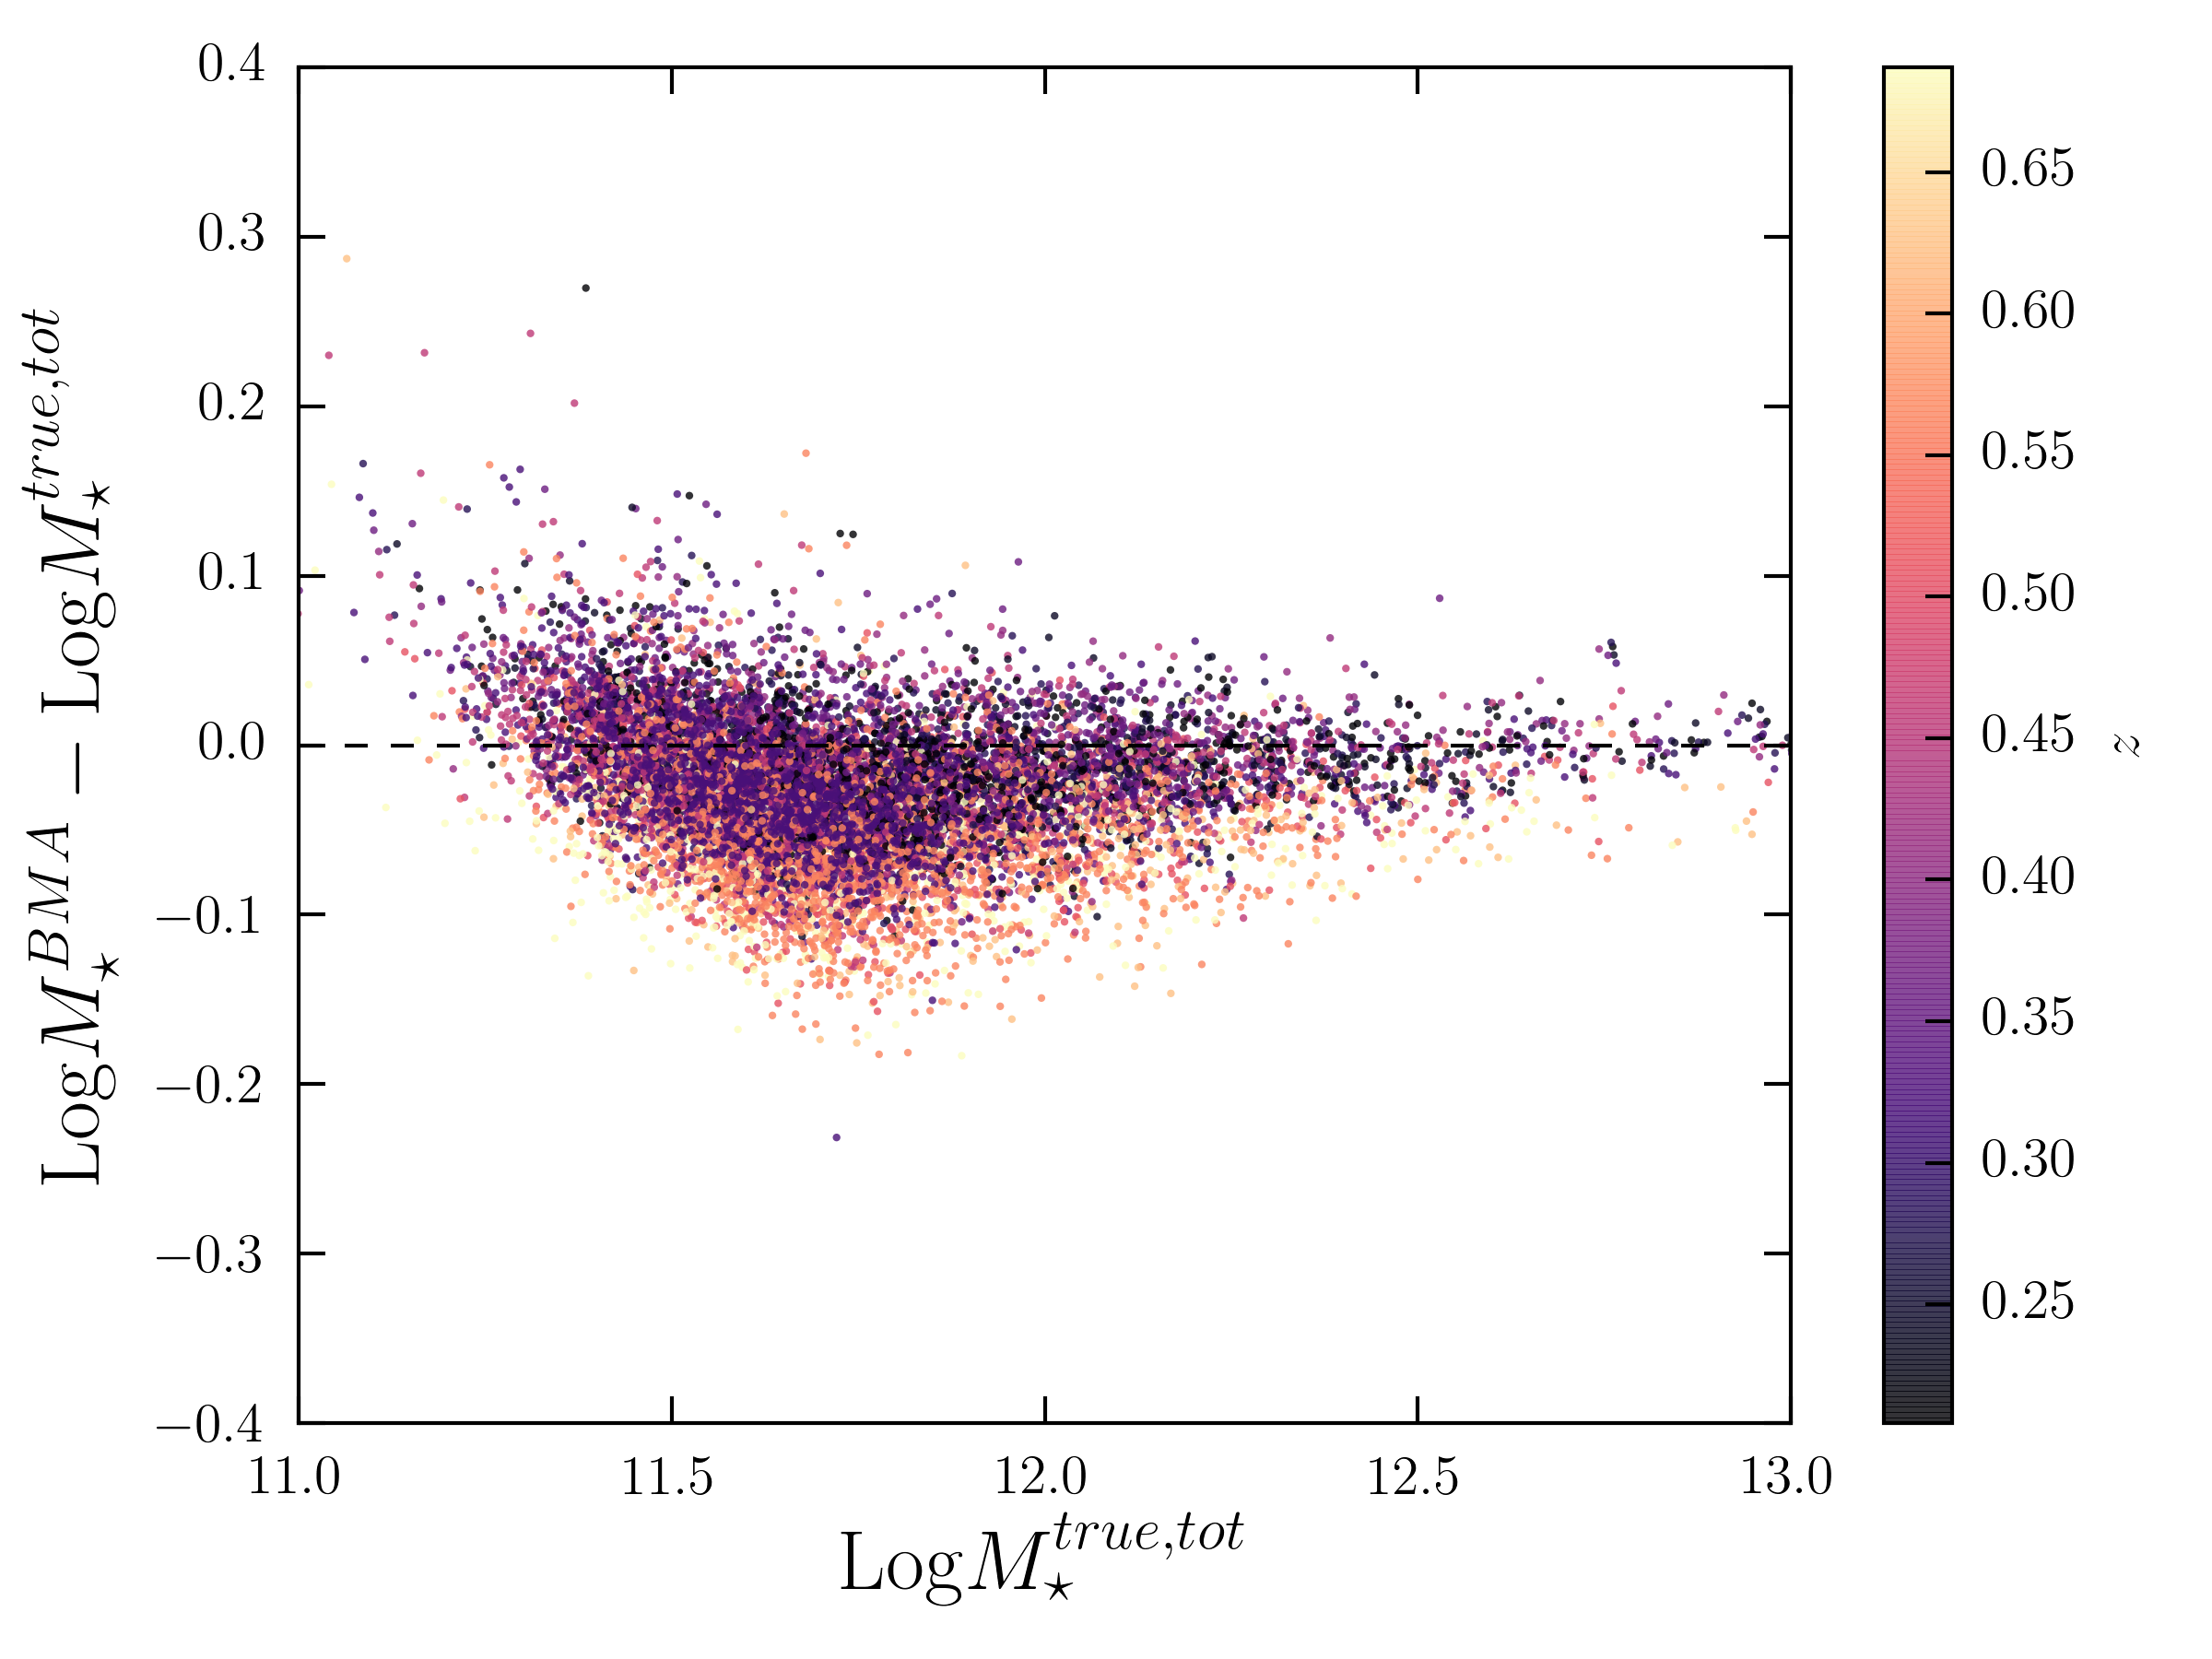
\includegraphics[width=0.7\textwidth]{./chapters/chapter5/figs/delucia_delta_clustersmass.png}\caption{Comparison of BMA clusters stellar mass to Millennium simulation true values at different redshifts. The dashed lines indicates no difference between the BMA estimates and the true values.}\label{fig:sims}\end{figure}

\subsubsection{The BMA method in clusters}
\citet{redmappersv} showed that  the redMaPPer photometric redshifts for DES  are excellent, with errors of the order $\sigma_z/(1+z)\sim 0.01$ up to $z\sim 0.9$. This allows us to safely assume the cluster redshift for the  cluster members and to avoid exploring the photo-z dependence of stellar masses, as was done in another DES study by \citet{capozzi}.
Despite the fact that in the present work we can safely  assume that the  cluster redshift is a good estimate of the real galaxy redshift, all the other  assumptions remain unconstrained.  We therefore choose not to ignore the uncertainty on model selection and use the BMA code presented in Chapter \ref{chp:sed} to estimate stellar masses and other properties of the single galaxies, from which we derive the total cluster stellar masses.
We test our results against the Millennium simulation semi-analytic model from \citet{delucia}\footnote{\url{http://gavo.mpa-garching.mpg.de/Millennium/Help?page=databases/millimil/delucia2006a}}, and show the results for the sum of stellar mass in clusters, in Figure \ref{fig:sims}. We run the BMA algorithm using the simulated magnitudes for the $griz$ SDSS filters, which are very similar to the DES ones. In this case the scatter of the bias distribution is even lower ($\lesssim 0.1$ dex) than what found in the comparison with the COSMOS results, showing that our method works well against other SED fitting methods and simulations. 

\begin{figure}\centering
 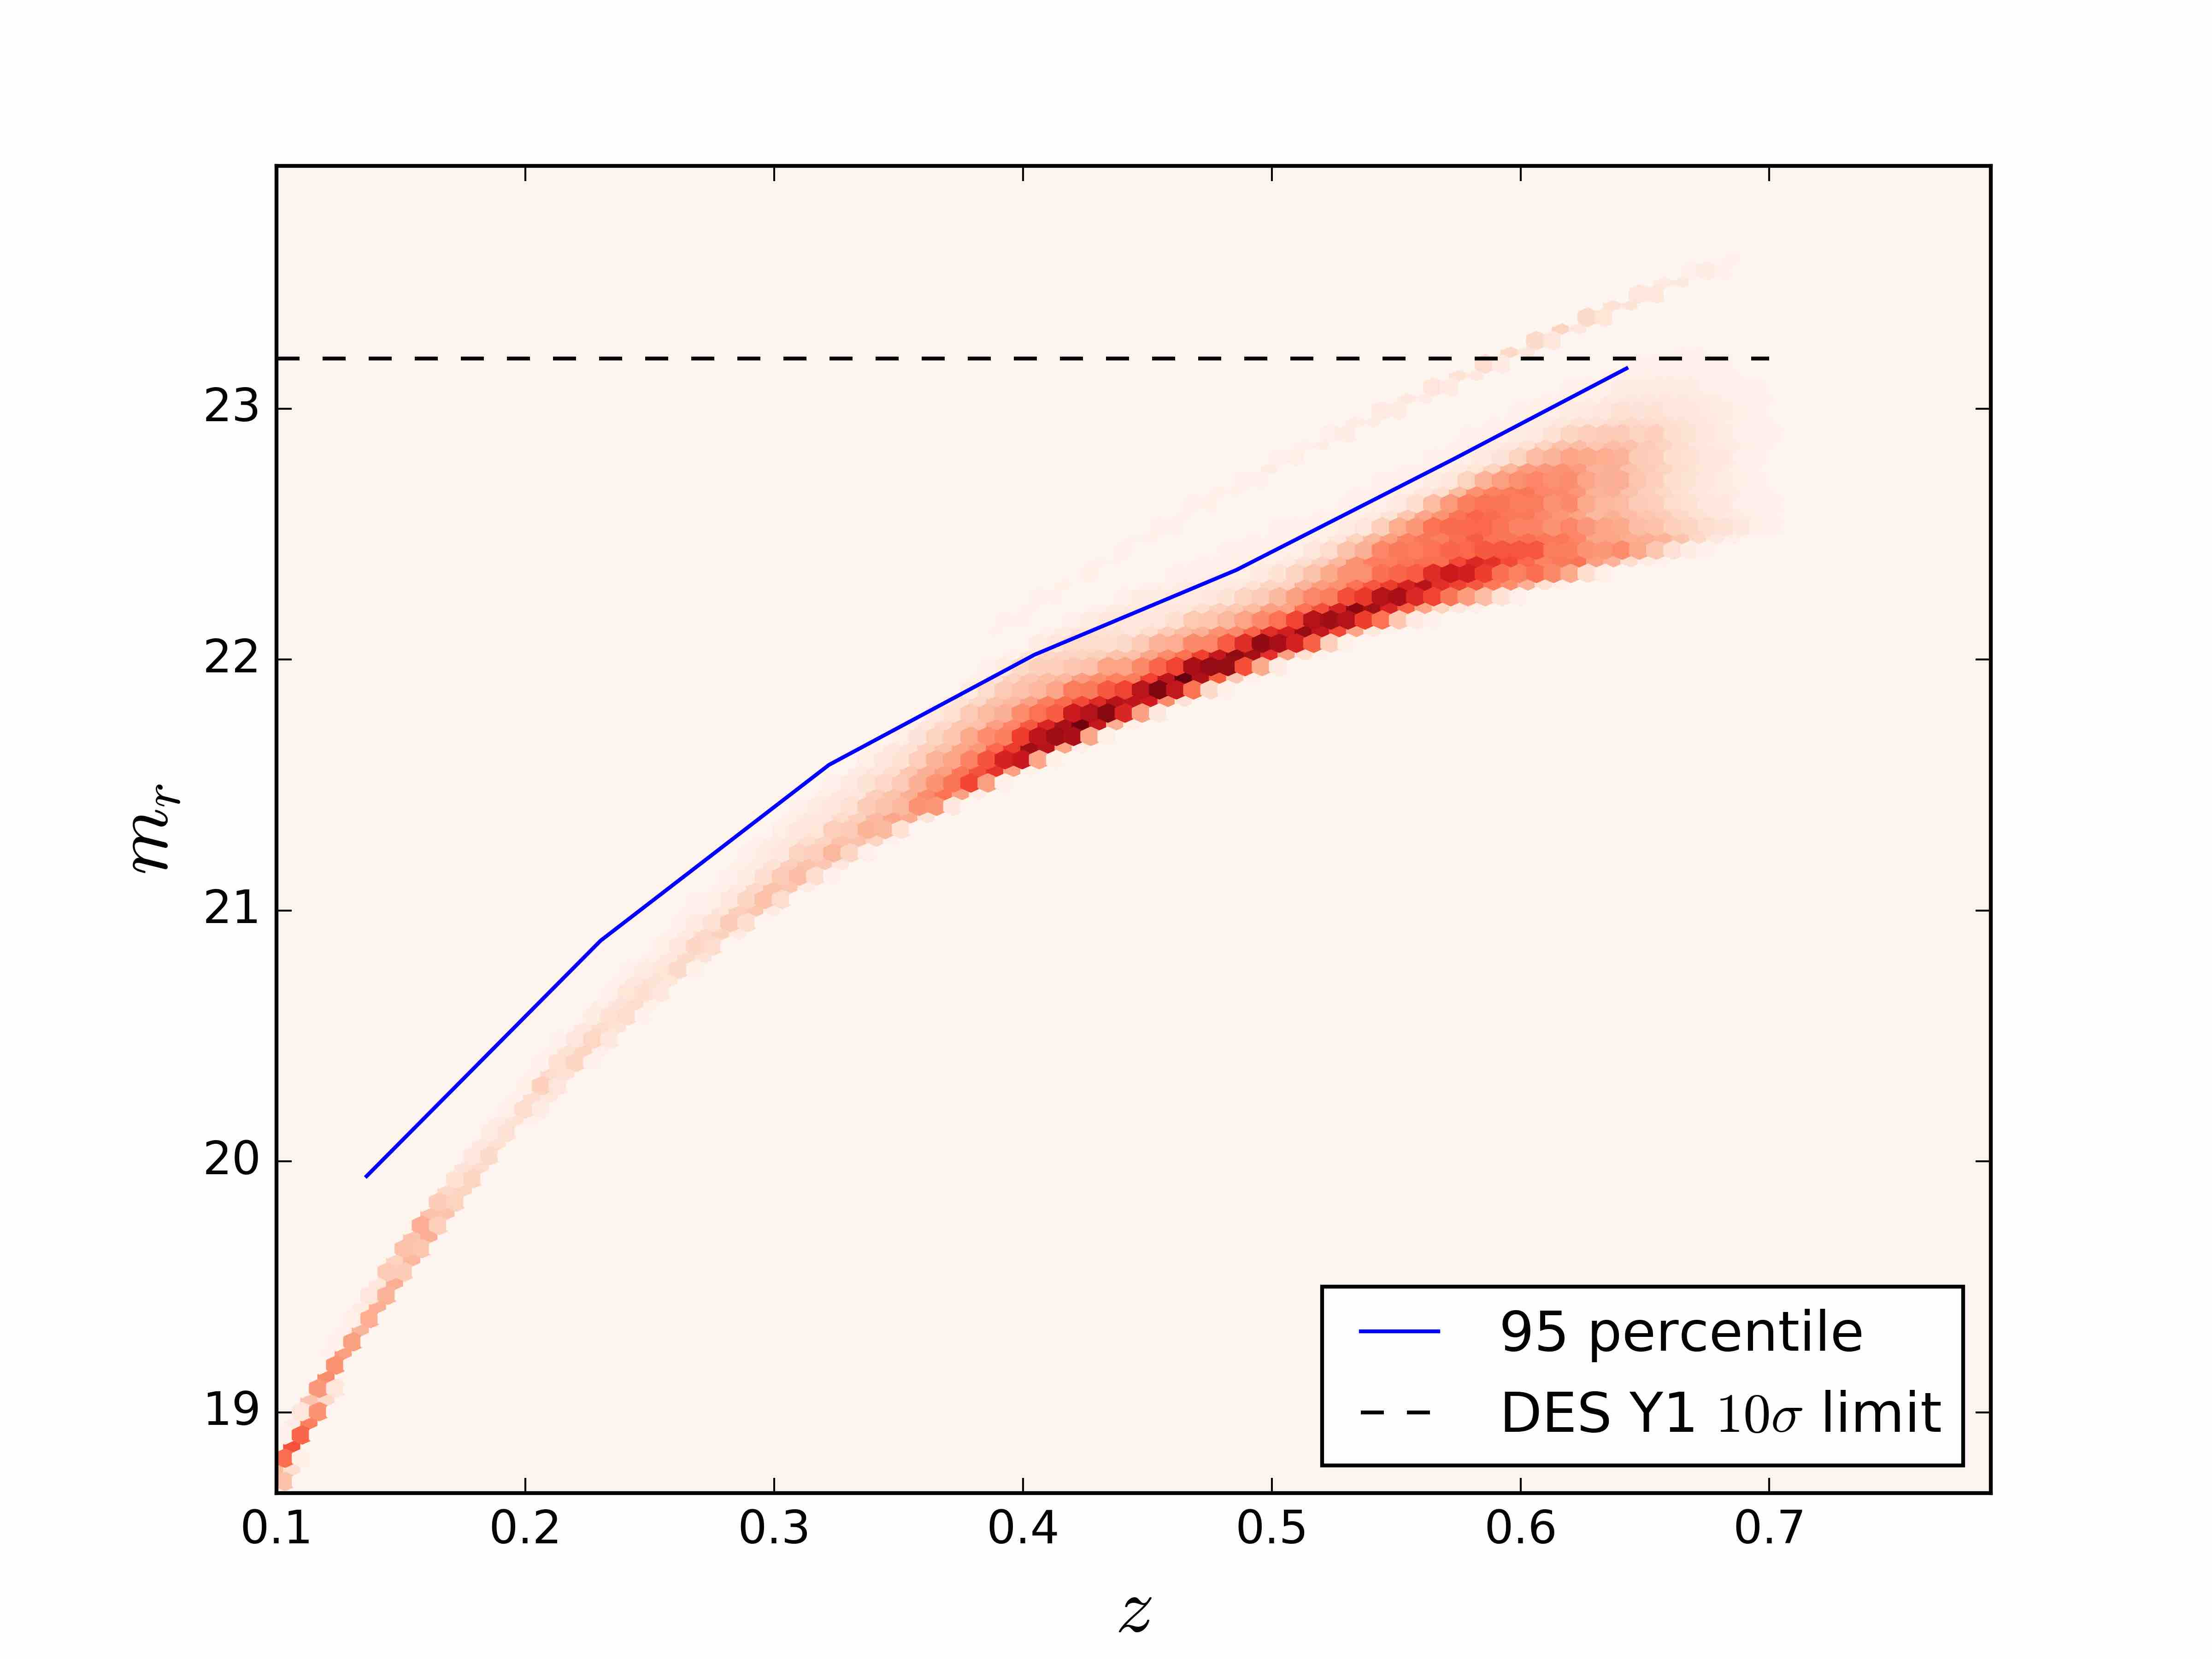
\includegraphics[width=0.7\textwidth]{./chapters/chapter5/figs/r_completeness.jpg}

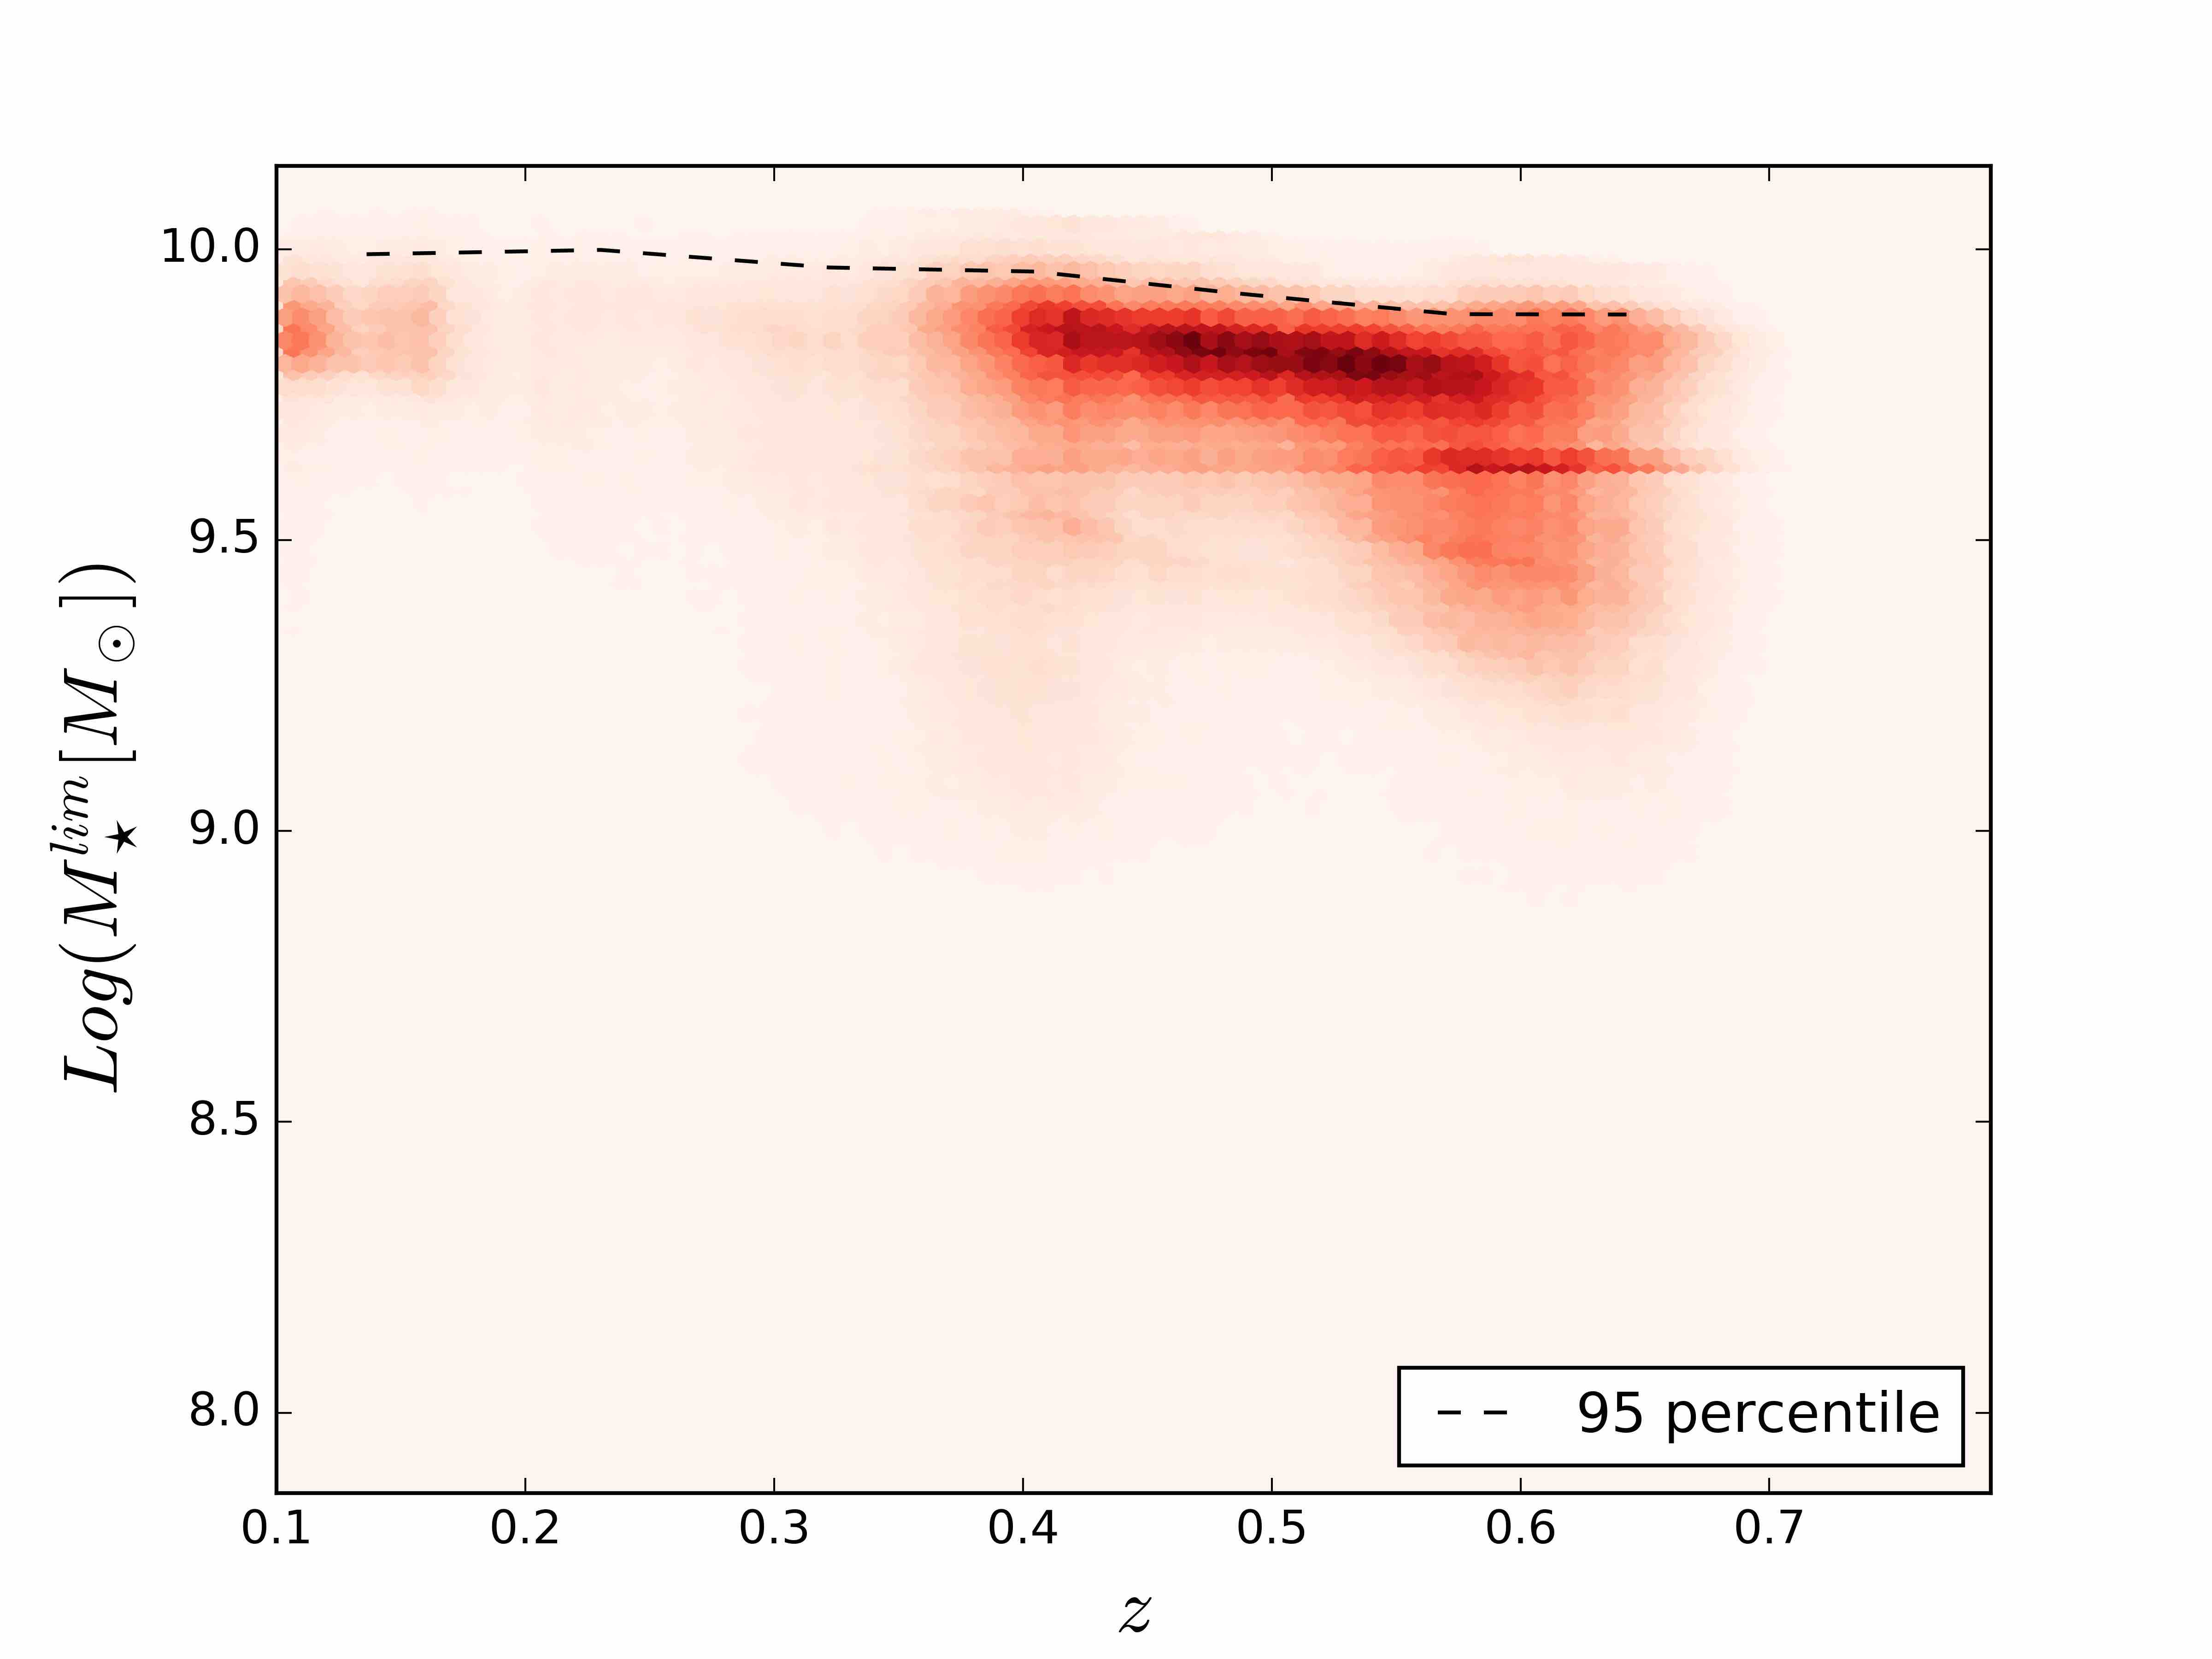
\includegraphics[width=0.7\textwidth]{./chapters/chapter5/figs/mass_completeness.jpg}\caption{Analysis of the completeness of the galaxy sample. \emph{Top panel:} observed $r$-band magnitudes that the galaxies in our sample would have if they had the absolute magnitude used as our limit ($M_r^{\rm lim} =-19$). The  95th percentile of the magnitude distribution lies below the median DES Y1 10$\sigma$ limit in $r$-band (dashed line).
\emph{Bottom panel:} limiting mass $M_\star^{lim}$ that each galaxy would have, at its redshift, if its absolute magnitude were equal to $M_r^{lim} =-19$. The limiting mass is below $10^{10}M_\odot$ at all redshifts; we therefor cut our sample at this stellar mass.}\label{compl}\end{figure}

\subsubsection{Completeness of the stellar mass sample}

The galaxy sample described in Section \ref{datasec} is cut at $M_r < -19$, where $M_r$ is the $r$-band absolute magnitude. Absolute magnitudes were estimated using K-corrections computed from galaxy templates generated by kcorrect v4.2 (\citealt{blanton}).  We took each galaxy's redshift to be the same as its photo-$z$, found the closest kcorrect template on a grid of redshift and colors ($g-r$, $r-i$, and $i-z$), and used that template's K-correction from observed $i$-band to rest-frame $r$-band to calculate $M_r$.  An absolute magnitude cut $M_r$ brighter than -19 was then applied to the galaxy catalog before computing membership probabilities. This cut ensures that our galaxy sample is  volume limited across the redshift range considered. In Figure \ref{compl} we show the observed $r$-band magnitudes that the galaxies in our sample would have if they had an absolute magnitude $M_r =-19$ as a function of redshift. These are computed using the $k$-corrections and distance modulus output by our BMA code for the galaxies with a membership probability $>8\%$, in order to be representative of a realistic cluster galaxy population. We show that the $95^{{\rm th}}$ percentile of the distribution in redshift bins is below the 10$\sigma$ limit of the Y1 DES catalog over the redshift range covered by the redMaPPer cosmology catalog. We compare to the Y1 magnitude limit as our galaxy catalog contains objects detected in Y1, even if they are matched to the deeper Y3 photometry. We can conclude that with the chosen cut we are always $\gtrsim 95\%$ complete.

%Note the Figures are actually for -19.5!!!

In order to estimate the completeness in stellar mass, we look at the mass $M_\star^{lim}$ each galaxy would have, at its redshift, if its absolute magnitude were equal to $M_r^{lim} =-19$. This can be achieved by converting the mass-to-light ratio fitted by BMA through $\log{(M_\star^{lim})} = \log{(M_\star)} + 0.4(M_r - M_r^{lim})$, where $M_r$ and $M_\star$ are the galaxy estimated absolute magnitude and stellar mass. From Figure \ref{compl} it is clear that, if all the galaxies were at $M_r^{lim}$ or fainter, $\gtrsim 95\%$ of them would have a stellar mass $\lesssim 10^{10} M_\odot$. We therefore are $\gtrsim 95\%$ complete above $M_\star =10^{10} M_\odot$ over the whole redshift range. The scatter in mass at each redshift is given by the scatter in $M/L$ of the different models. We therefore cut our stellar mass sample at $M_\star >10^{10} M_\odot$.

\subsection{From galaxy stellar masses to $\mu_\star$}\label{tomustar}

The cluster mass proxy $\mu_\star$ is computed by weighing the stellar mass of each galaxy in the cluster by its membership probability $p_{{\rm mem}, i}$:
\begin{equation}
\mu_\star = 10^{-10} M_\odot^{-1} \sum_i  p_{{\rm mem}, i} M_{\star,i}\,,\label{eq:mustar}
\end{equation}
where the factor $10^{-10}$ simply gives to the mass proxy an order of magnitude similar to that of the number of observed cluster galaxies. The sum is over all the galaxies from the DES Y1A1 gold catalog having $M_r<-19$ and within 3 Mpc from the centre of the cluster as given by the redMaPPer Y1 catalog. The errors on $\mu_\star$ were computed using jackknife resampling. Intuitively, this method allows us to estimate the variance on our estimator by considering a galaxy cut from the cluster at each time.

\subsubsection{Membership probability assignment}

The membership probability for a galaxy in a cluster is given by
\begin{equation}
p_{\rm mem} = p_{R}\,p_{z}\,,\label{eq:pmem}
\end{equation}
where the components represent the probability of the galaxy being a member given its redshift ($p_z$) and its projected distance from the cluster center ($p_R$). The radial probability $p_R$ is assigned by assuming a projected Navarro--Frenk--White (NFW; \citealt{nfw}) profile, with $R_{200c}$ computed by counting galaxies within 3 Mpc and finding the halo profile by assuming an Halo Occupation Distribution model. Useful information is also contained in the color probability. In order to assign these probabilities to each galaxy in a cluster, we therefore need to complete the following steps:

\begin{enumerate}
\item {\bf Assign redshift probabilities. } By assuming that each galaxy redshift follows a Gaussian probability density function (PDF) with the mean being the observed photometric redshift $z$ and the standard deviation being the uncertainty in the photometric redshift $\delta z$, we define the probability as the integral of the redshift PDF over a window around the redshift of the cluster $z_0$:
\begin{equation}
p_z=\int_{z_{min}}^{z_{max}} \frac{1}{\sqrt{2\pi}(\delta z')}e^{-\frac{(z'-z_{0})^2}{2 (\delta z') ^2}}dz'\, .
\end{equation}
In general, photo-$z$ PDFs are not Gaussian. However, full PDFs are not available for Y3 data, so this is our best estimate.
In order to account for changing photometric redshift uncertainties at different redshifts, we evolve the size of the window with redshift based on the median photometric redshift uncertainty $\langle \delta z \rangle$ of galaxies in our sample at a given redshift. The bounds of our integral $z_{min}$ and $z_{max}$ are defined to evolve as  
\begin{gather}
\nonumber z_{min}=z_{0}-\langle \delta z \rangle \\
z_{max}=z_{0}+\langle \delta z \rangle
\end{gather}
This redshift probability gives galaxies of approximately the same redshift as the cluster center a greater weight than galaxies at vastly different redshifts. 

\item {\bf Count galaxies}. We count all galaxies along the line of sight within circular apertures with radii $0.1\leq r \leq 3.0$ Mpc, weighted by $p_z$. This effectively selects galaxies near the cluster redshift while avoiding a sharp, arbitrary cutoff in redshift. The redshift weighted galaxy number counts as a function of radius are divided by the surface area at each radius. This converts our number counts into a surface density, which is background--subtracted. 

\item {\bf Background subtraction. } Background or foreground galaxies are likely to enter into our number counts. To remove this contribution, we measure a local background galaxy density in the environment around each cluster. Similarly to the previous step, this contribution is estimated by summing the photo-$z$ probability weighted galaxy counts in an annulus around the cluster. We choose the internal radius of this annulus to be 4 Mpc in order to be far enough away from the cluster virial radius. The outer radius was chosen to be 6 Mpc to provide a sizable area to smooth out small fluctuations in density. The derived profile is transformed into a surface density and subtracted from the cluster surface density.

\item {\bf Convert from a number density of galaxies to a mass density}. This step is performed by assuming the HOD model of \cite{Tinker2011CosmologicalClusters}. 
%This model provides a two part halo occupation function, with one piece representing the central galaxy occupation and the other representing the satellite galaxy occupation. The occupation function for central galaxies takes the form 
%\begin{equation}
%\langle N_{cen} \rangle_M = \frac{1}{2} \Bigg[1+\erf \Bigg(\frac{\log M - \log M_{min}}{\sigma_{\log M}}\Bigg)\Bigg]
%\end{equation}
%where $M_{min}$ represents the halo mass at which the probability of containing a central galaxy is $50\%$, and $\sigma_{\log M}$ accounts for the scatter in halo mass at a fixed luminosity. The occupation function for satellites is defined to be 
%\begin{equation}
%\langle N_{sat} \rangle_M = \langle N_{cen} \rangle_M \times \Bigg(\frac{M}{M_{sat}}\Bigg)^{\alpha_{sat}} \exp{\Bigg(\frac{-M_{cut}}{M}\Bigg)}.\end{equation}
%This models the satellite occupation distribution as a power law with a slope given by $\alpha_{sat}$ at high halo masses, with an exponential cutoff at halo masses below $M_{cut}$. Combining the central and satellite occupation functions produces a total occupation function of the form 
%\begin{equation}\langle N_{tot} \rangle_M = \langle N_{cen} \rangle_M \times \Bigg[1 + \Bigg(\frac{M}{M_{sat}}\Bigg)^{\alpha_{sat}} \exp{\Bigg(\frac{-M_{cut}}{M}\Bigg)}\Bigg].\end{equation}
%\cite{Tinker2011CosmologicalClusters} perform a fit to several sets of parameter values for their model (which are given in their Table 4). One of the fits they perform corresponds to an absolute magnitude limit of $M<-19.5$. Because this magnitude limit corresponds to our own magnitude limit, we can use the parameter values they provide, and thus avoid having to calculate our own fits. This greatly simplifies our analysis. 
%\item Estimate $R_{200c}$. The HOD model provides a number of galaxies as a function of halo mass, however we want to perform the opposite conversion for our analysis. To do this, we interpolate the $N_{tot}$ function over a range of masses spanning the below expected mass of a single galaxy to beyond the largest mass observed for a cluster. This allows us to numerically convert our background subtracted galaxy number counts as a function of radius into mass as a function of radius, and then into a mass density as a function of radius. 
We interpolate the background subtracted cluster mass density within our apertures to find where the density equals 200 times the critical density, thus giving our value of $R_{200c}$. 

\item {\bf Assign radial probabilities.} Our radial probability assume a projected NFW mass profile, of the form \citep{Wright2000GRAVITATIONALHALOS}:

\begin{equation}
\Sigma (R) = \begin{cases}
\frac{2\rho_s R_s}{r^2-1} \Big[1-\frac{2}{\sqrt{r^2-1}}{\rm arctan} \sqrt{\frac{r-1}{r+1}} \Big] & r>1 \\
\frac{2\rho_s R_s}{3} & r=1 \\
\frac{2\rho_s R_s}{r^2-1} \Big[1-\frac{2}{\sqrt{1-r^2}}{\rm arctanh} \sqrt{\frac{1-r}{r+1}} \Big] & r<1 \\
\end{cases}\label{eq:sigma}
\end{equation}

where $r=R/R_s$, and $R_s=R_{200c}/c$ is the scale radius, with $c$ being the concentration parameter set to $c=3$. %In order to avoid the singularity at $R=R_s$ we set a core radius $R_{\rm core}=R_s$, and we approximate the density inside this core radius as constant.

The radial probability is computed from Eq. (\ref{eq:sigma}) as:
\begin{equation}
p_R=\frac{k \Sigma (R)}{k \Sigma (R) + \Sigma_{\rm bg}} \, ,
\end{equation}
 where $k$ is a constant given by the background subtracted surface number density $n_{\rm tot}-n_{\rm bg}$ and $\Sigma_{\rm bg}$ is the background surface density.
 %\begin{equation}k=\frac{n_{tot}-n_{bg}}{\int_0^{R_{200}}{2 \pi R' \Sigma (R')} dR'}\end{equation}

\begin{figure}\centering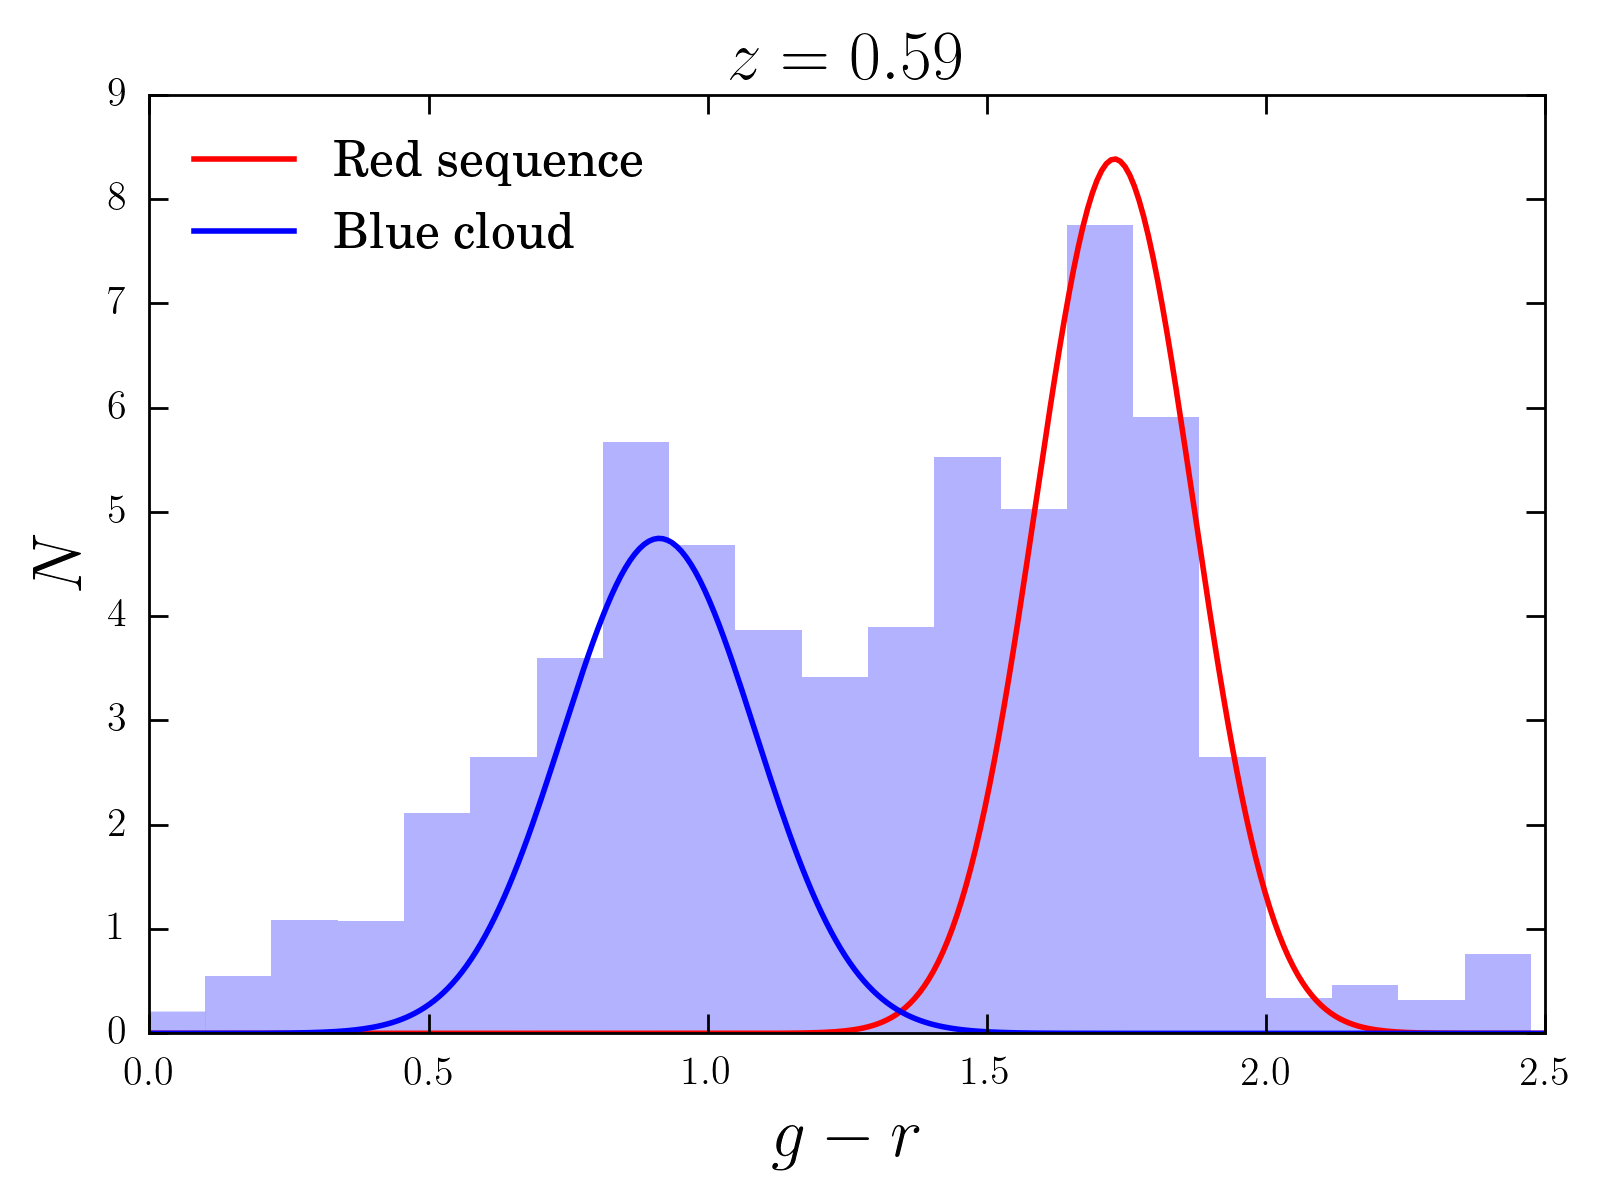
\includegraphics[width=0.7\textwidth]{./chapters/chapter5/figs/cl_test.png}
\caption{Colour distribution in $g-r$ of a cluster at $z=0.59$ from the Y1 redMaPPer sample, given as an example. The histogram is made by counting all galaxies within 3 Mpc of the cluster center, weighted by their membership probability. The red and blue Gaussians represent the best fit of the red sequence and blue cloud from the Gaussian Mixture Model after background subtraction.}\label{fig:histcl}\end{figure}

\item {\bf Assign colour probability.} Colour probabilities $p_{\rm c}$ are estimated through a Gaussian Mixture Model (GMM), similarly to \citet{Hao2009PRECISIONMODEL}. The fit is performed using a modified version of \texttt{scikit-learn} Python package \citep{Pedregosa2011Scikit-learn:Python}. This method fits two Gaussians to the colour distribution of the galaxies in each cluster, weighted by their radial and redshift probabilities. The Gaussians fit the color distribution of the red sequence and blue cloud of cluster galaxies well. Figure \ref{fig:histcl} shows the two Gaussians for a randomly selected cluster from the Year 1 redMaPPer sample. A Gaussian PDF for the probability that a galaxy would have color $x$ given it is in a color distribution of mean colour $\mu$ and variance $\sigma^2$ can be written as:
\begin{equation} 
p(x | \mu,\sigma^2)= \frac{1}{\sqrt{2\pi\sigma^2}}e^{-\frac{(x-\mu)^2}{2\sigma ^2}} \,.
\end{equation} 
We define a colour probability density that a galaxy with color $x$ is a member of a cluster with red and blue Gaussian color distribution given by $\mu_r,\sigma_r$ and $\mu_b,\sigma_b$ from the GMM fit as:
\begin{equation}
\Pi(x)=w_r p(x | \mu_r,\sigma_r^2) + w_b p(x | \mu_b,\sigma_b^2)\,, \label{eq:pc}
\end{equation}
where $w_{r}$ and $w_{b}$ are the area of the Gaussians and satisfy $w_{ r}+w_{b}=1$. %Next, we compute a constant of normalization
%\begin{equation}
%\kappa=\sum_i{\bigg(N_{tot}(x_i)-N_{bg}(x_i)\bigg)}
%5\end{equation}
Finally, we compute the probability that the galaxy is in the cluster given its colour:
\begin{equation} 
p_{\rm c}=\frac{\kappa \Pi (x)} {\kappa \Pi (x) + N_{\rm bg}(x)}\, ,
\end{equation} 
where $\kappa$ is the background--subtracted number of galaxies.
%Nsubtracted is the number of cluster galaxies remaining after the background subtraction. 
We can also define the probability of being in the red sequence:
\begin{equation}
P({\rm RS}|x)=\frac{\kappa \Pi_{\rm RS}(x)} {\kappa \Pi_{\rm RS}(x) + N_{bg}(x)}\, ,\label{eq:prs}
\end{equation}
where
\begin{equation}
\Pi_{\rm RS}(x)=w_r p(x | \mu_r,\sigma^2_r)\, .
\end{equation}
These probabilities are computed for the available colors $g-r$, $r-i$, and $i-z$.
\end{enumerate}

\section{Calibrating $\mu_\star$ against X-ray mass observables}\label{calibsec}

\subsection{The $T_X-\mu_\star$ relation}
Following previous works (e.g. \citealt{rozo09}; \citealt{extrinsicscatter}; \citealt{mulroy}), we perform a Bayesian linear regression of the scaling relation between the logarithm of the X-ray mass proxy (in this case the temperature $T_X$) and the logarithm of our photometric mass proxy, including an intrinsic scatter $\sigma_{{\rm Log} T_X|\mu_\star}$ of the temperature at fixed $\mu_\star$. A Bayesian linear regression assumes Bayes' theorem in its formalism, and we choose this method because it easily allows the inclusion of an intrinsic scatter. The formalism is presented in Section \ref{shmrsec} for a more generic case, where we will need to include an extra variable in the fit which is not permitted in publicly available routines. Namely, we fit:
\begin{equation}
\langle {\rm Log}~ T_X|\mu_\star\rangle = \alpha+\beta~{\rm Log}\Big( \frac{\mu_\star}{\tilde{\mu_\star}} \Big)\, ,\label{eq:tx}
\end{equation}
where  $\tilde{\mu_\star}=1000$ is roughly the mean $\mu_\star$ of the sample. We use the publicly available Python version of \citealt{kelly} and separately fit the X-ray temperatures presented in Section \ref{sec:xray} for the \emph{XMM} and \emph{Chandra} samples. We perform separate fits for the two samples as combining different temperature measurements is not straightforward and we are not interested in fitting a generic $T_X-\mu_\star$ relation but rather to test our methodology against other well established mass proxies.
The results of the regression are reported in Table \ref{tab:tx} and shown in Figure \ref{fig:tx}. The slope found for the \emph{Chandra} temperatures is shallower ($\beta=0.295^{+0.070}_{-0.071}$) because the dynamical range explored by $T_X$ is not as wide as in the \emph{XMM} sample and some cluster temperatures have a very low signal-to-noise in the low $T_X$ and low $\mu_\star$ end regimes (thus they are cut by our SNR selection). \citet{farahi} also find a shallower slope in the $T_X-\lambda$ relation for the \emph{Chandra} sample matched to Y1 redMapper clusters. The mass proxy seems to correlate better with the \emph{XMM} temperatures, resulting in a slope of $\beta=0.483\pm 0.053$. 

The weak lensing mass--$\mu_\star$ relation studied in \citet{maria} and presented in Section \ref{wlcalib} shows a steeper slope ($1.74\pm 0.62$ at $0.1<z<0.33$ for SDSS redMaPPer clusters) than the analysis presented here. We believe that the correlation of stellar mass with total cluster mass is higher than with the X-ray temperatures because the X-ray measurement only probes the inner part of the cluster gravitational potential (within $R_{500c}$ and $R_{2500c}$ for the \emph{XMM} and \emph{Chandra} data respectively), while the weak lensing probes larger radii.

We perform the same linear regression of Eq. (\ref{eq:tx}) with the X-ray luminosities in units of $10^{44} {\rm erg/s}$ in place of the temperatures. Results are reported in Table \ref{tab:tx}. We find a larger scatter for this relation, which is expected as the temperature directly probes the potential well of the halo, while the luminosity depends primarily on the density of the Intra--cluster Medium (ICM). This causes baryon effects to be included to a higher order and the scatter with halo mass to increase.
%{\bf Compare the fitting results with $M_{200}$ to other studies (see  section  3.1 of van Uitert et al 2016) Compare to WL scaling relations in \citet{maria}, \citet{melchior}, \citet{mulroy}}

\begin{table}\centering
\begin{tabular}{c|ccc}
\hline
\hline
 Sample--observable &$\alpha$&$\beta$&$\sigma_{{\rm Log} T/L_X|\mu_\star}$\\
 \hline
\emph{XCS}--$T_X$ & $0.580^{+0.021}_{-0.021}$ & $0.483^{+0.053}_{-0.053}$ & $0.152^{+0.017}_{-0.015}$\\
\emph{XCS}--$L_X$ & $0.392^{+0.064}_{-0.065}$ & $1.54^{+0.18}_{-0.17}$ & $0.514^{+0.051}_{-0.047}$\\
%\emph{Chandra}--$T_X$ & $0.821^{+0.019}_{-0.020}$ & $0.182^{+0.065}_{-0.065}$ & $0.120^{+0.014}_{-0.012}$\\
\emph{Chandra}--$T_X$ & $0.784^{+0.022}_{-0.022}$ & $0.295^{+0.070}_{-0.071}$ & $0.139^{+0.015}_{-0.014}$\\
\emph{Chandra}--$L_X$ & $0.644^{+0.062}_{-0.062}$ & $0.84^{+0.20}_{-0.20}$ & $0.436^{+0.040}_{-0.037}$\\
\end{tabular}\caption{Fits of the scaling relation following Eq.(\ref{eq:tx}) for X-ray temperatures and luminosities. Values represent the median of the parameters posterior distribution, and the errors are the 16th and 84th percentiles. Temperatures are in units of keV and luminosities in $10^{44} {\rm erg s^{-1}}$}\label{tab:tx}
\end{table}

\begin{figure}\centering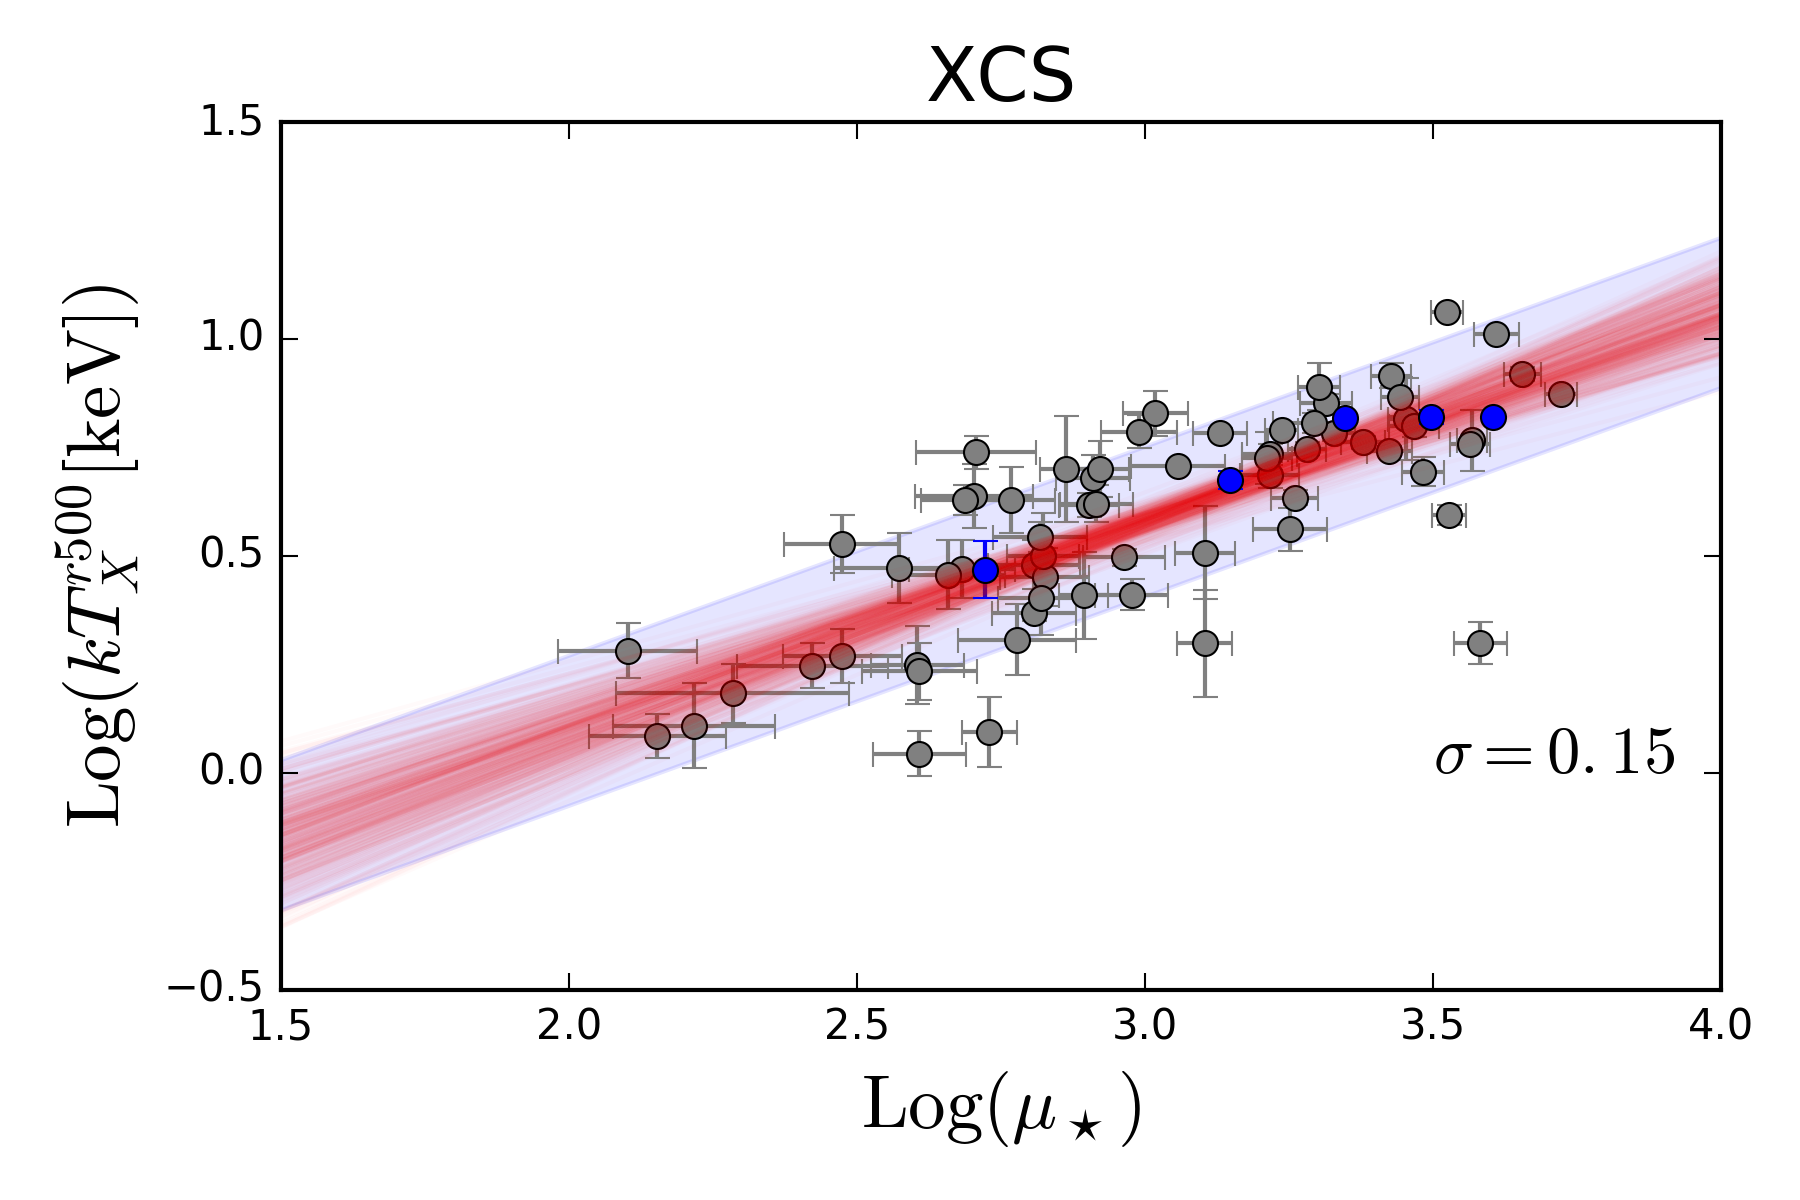
\includegraphics[width=0.7\textwidth]{./chapters/chapter5/figs/xmm_mu_scatter.png}
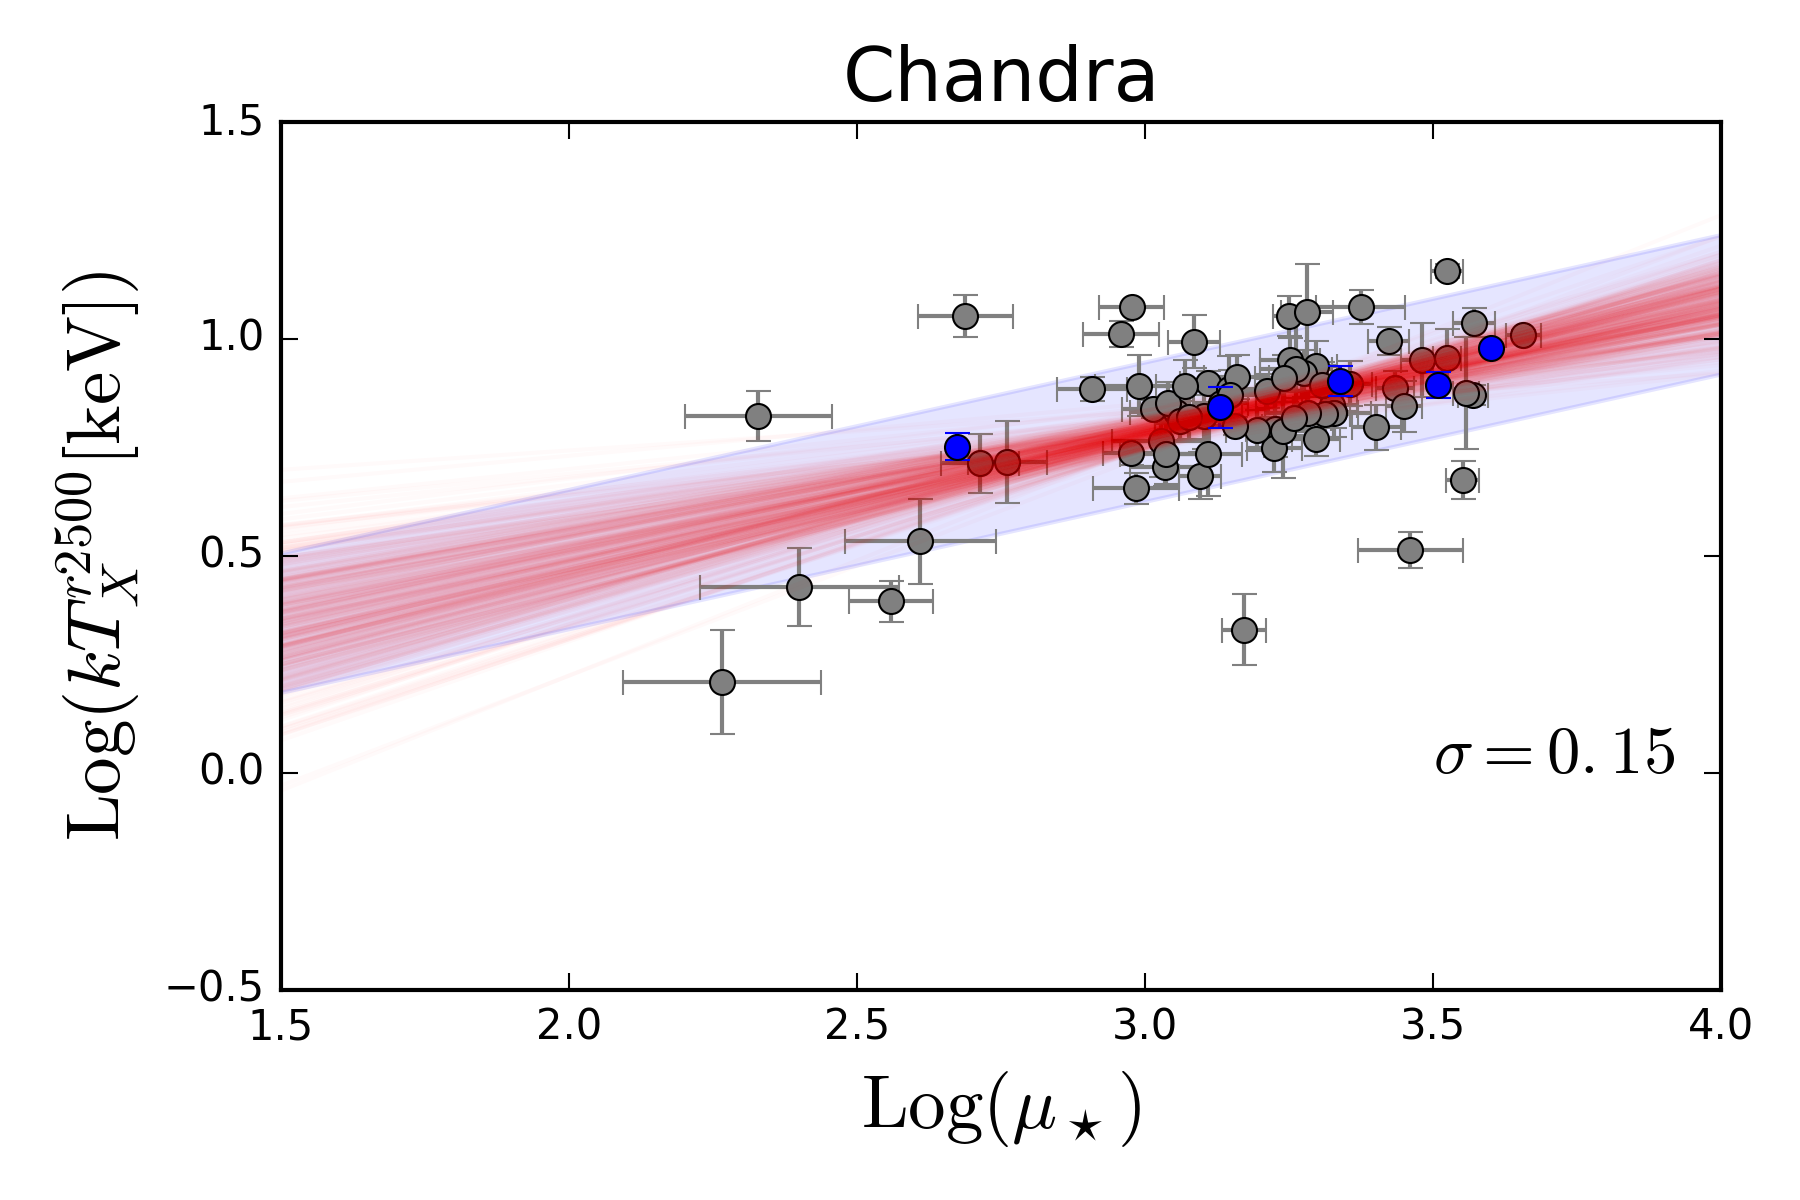
\includegraphics[width=0.7\textwidth]{./chapters/chapter5/figs/chandra_r2500_mu_iz_scatter.png}\caption{Bayesian linear regression of $X$-ray temperature and $\mu_\star$ for the XCS high signal-to-noise sample (top panel) and the Chandra sample (bottom panel). The grey points are our sample data points, the blue points are the mean temperature and mass proxy values in $\mu_\star$ bins. The red lines are a random sample from the posterior distribution of slope and intercept, and the blue band represents 1$\sigma$ around the mean value of the intercept plus the intrinsic scatter.}\label{fig:tx}\end{figure}


\begin{figure}
\centering
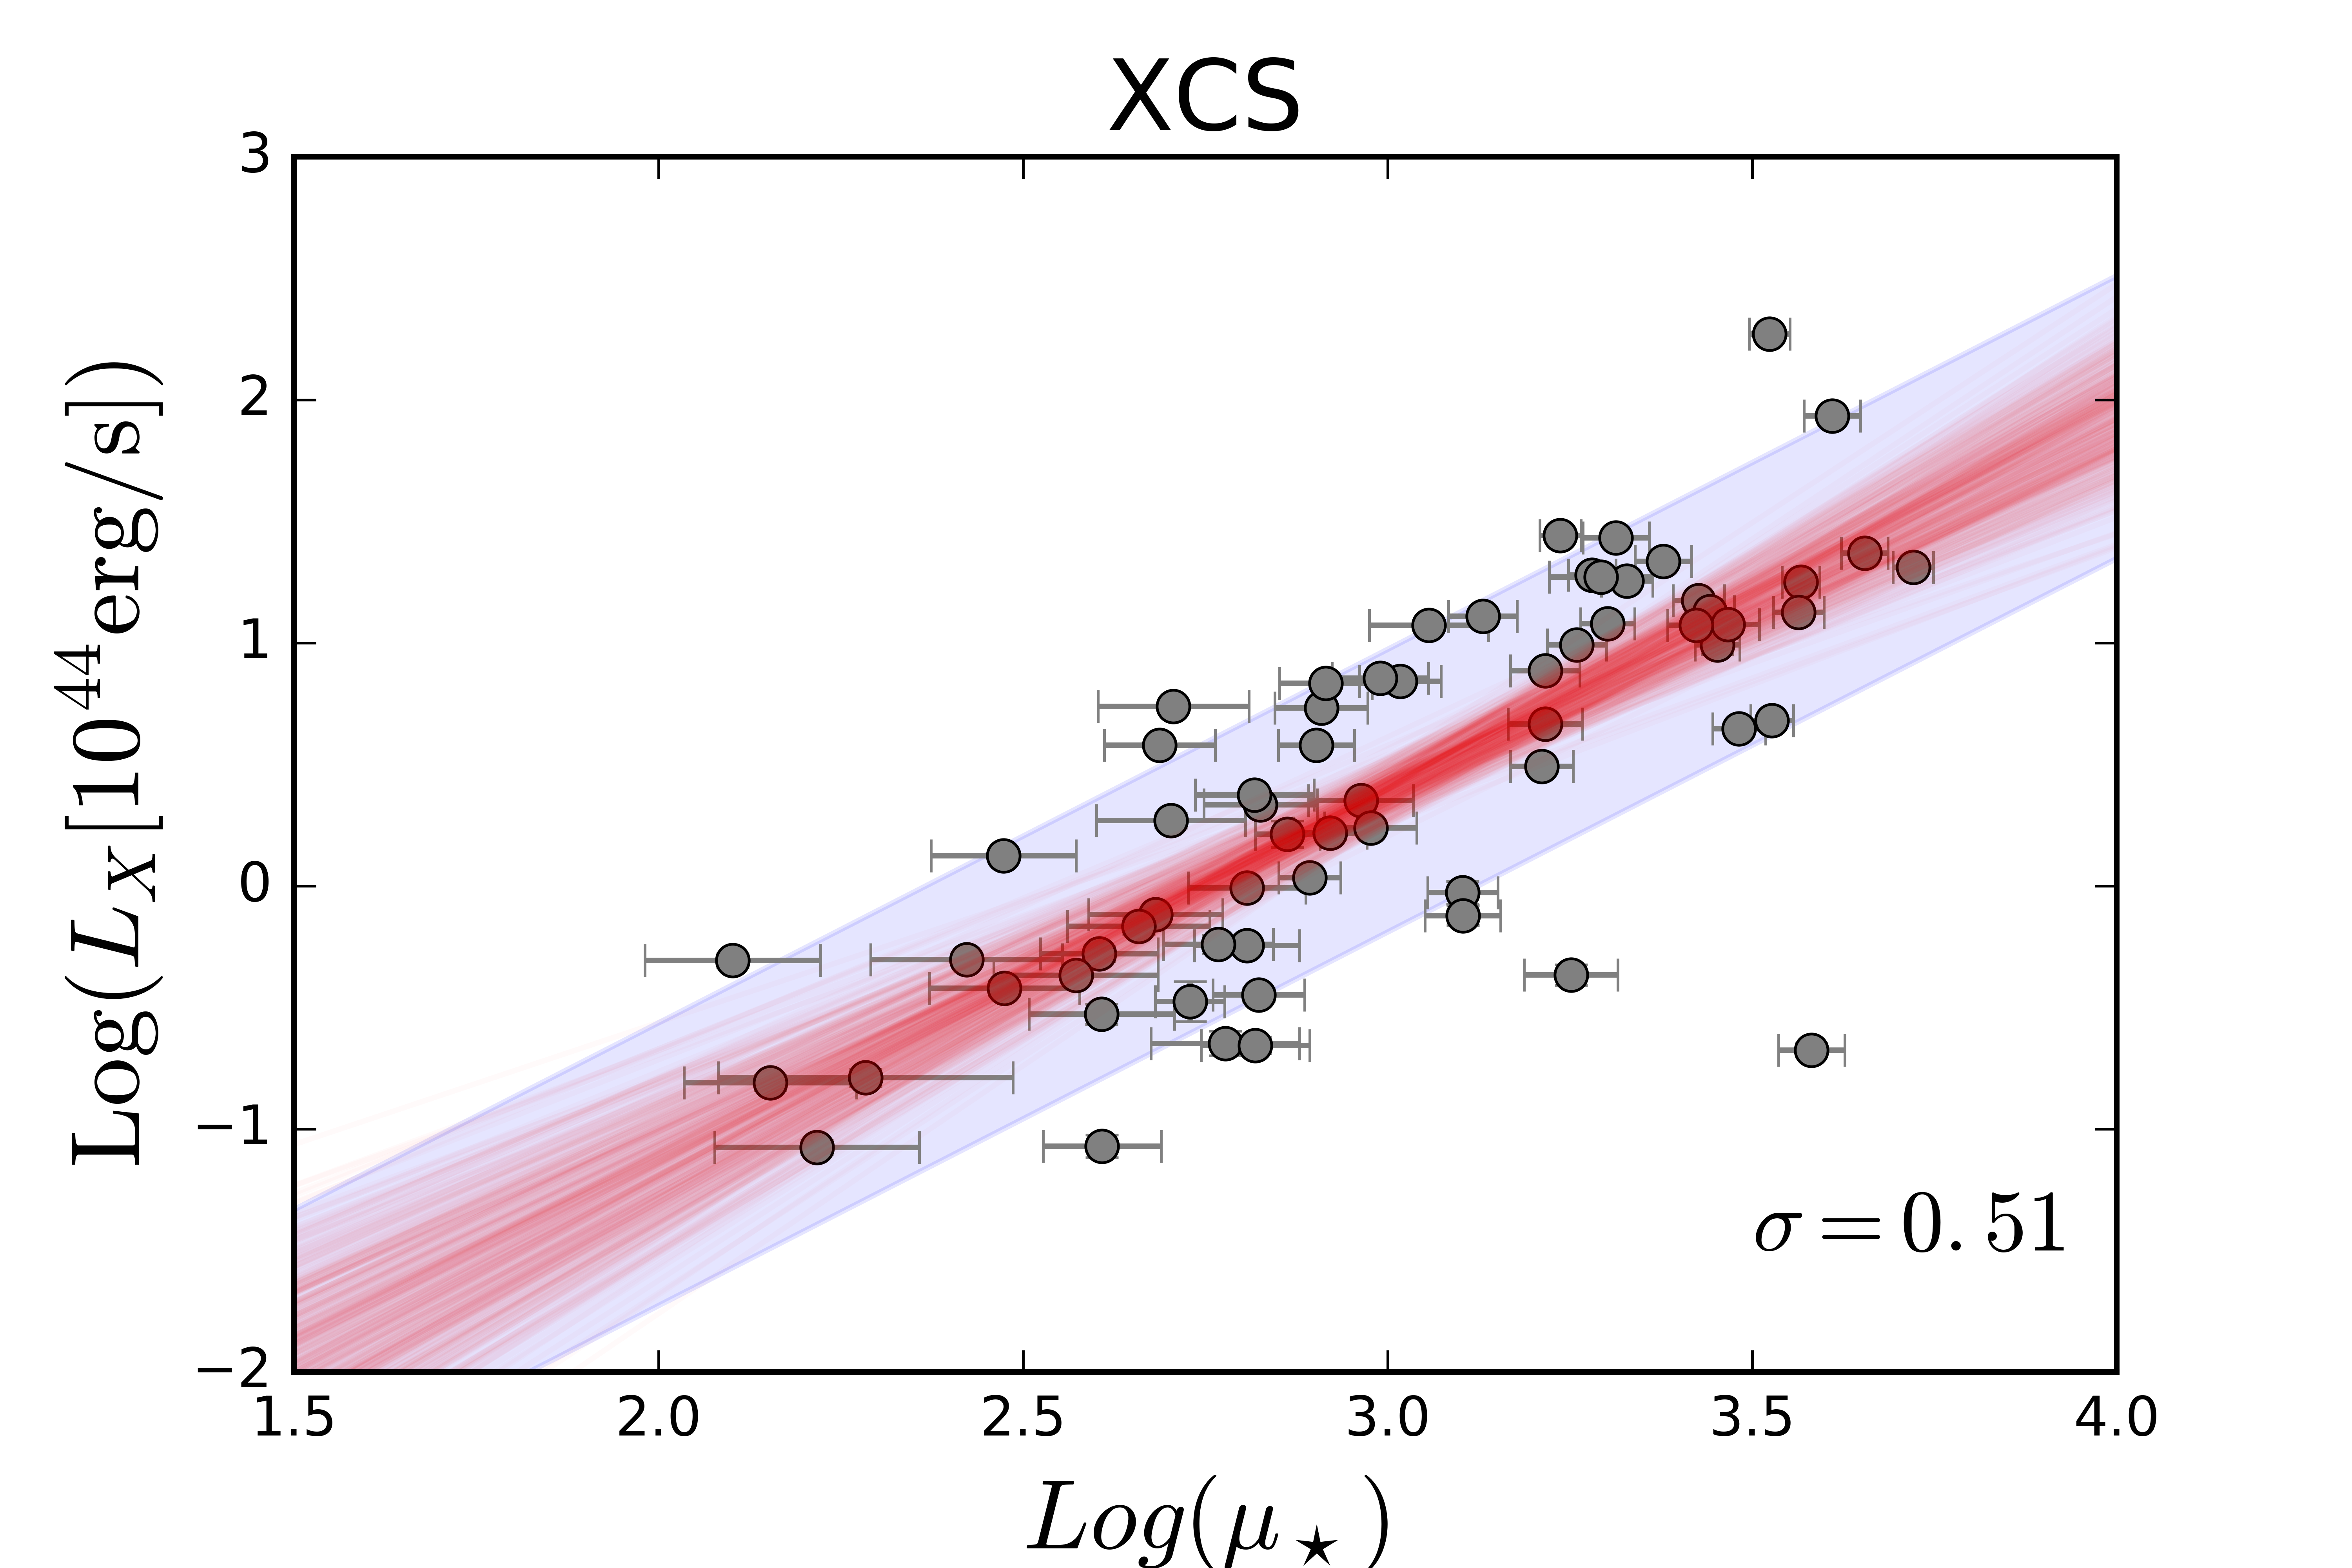
\includegraphics[width=0.7\textwidth]{./chapters/chapter5/figs/xmm_lx_mu_scatter_Feb18.png}
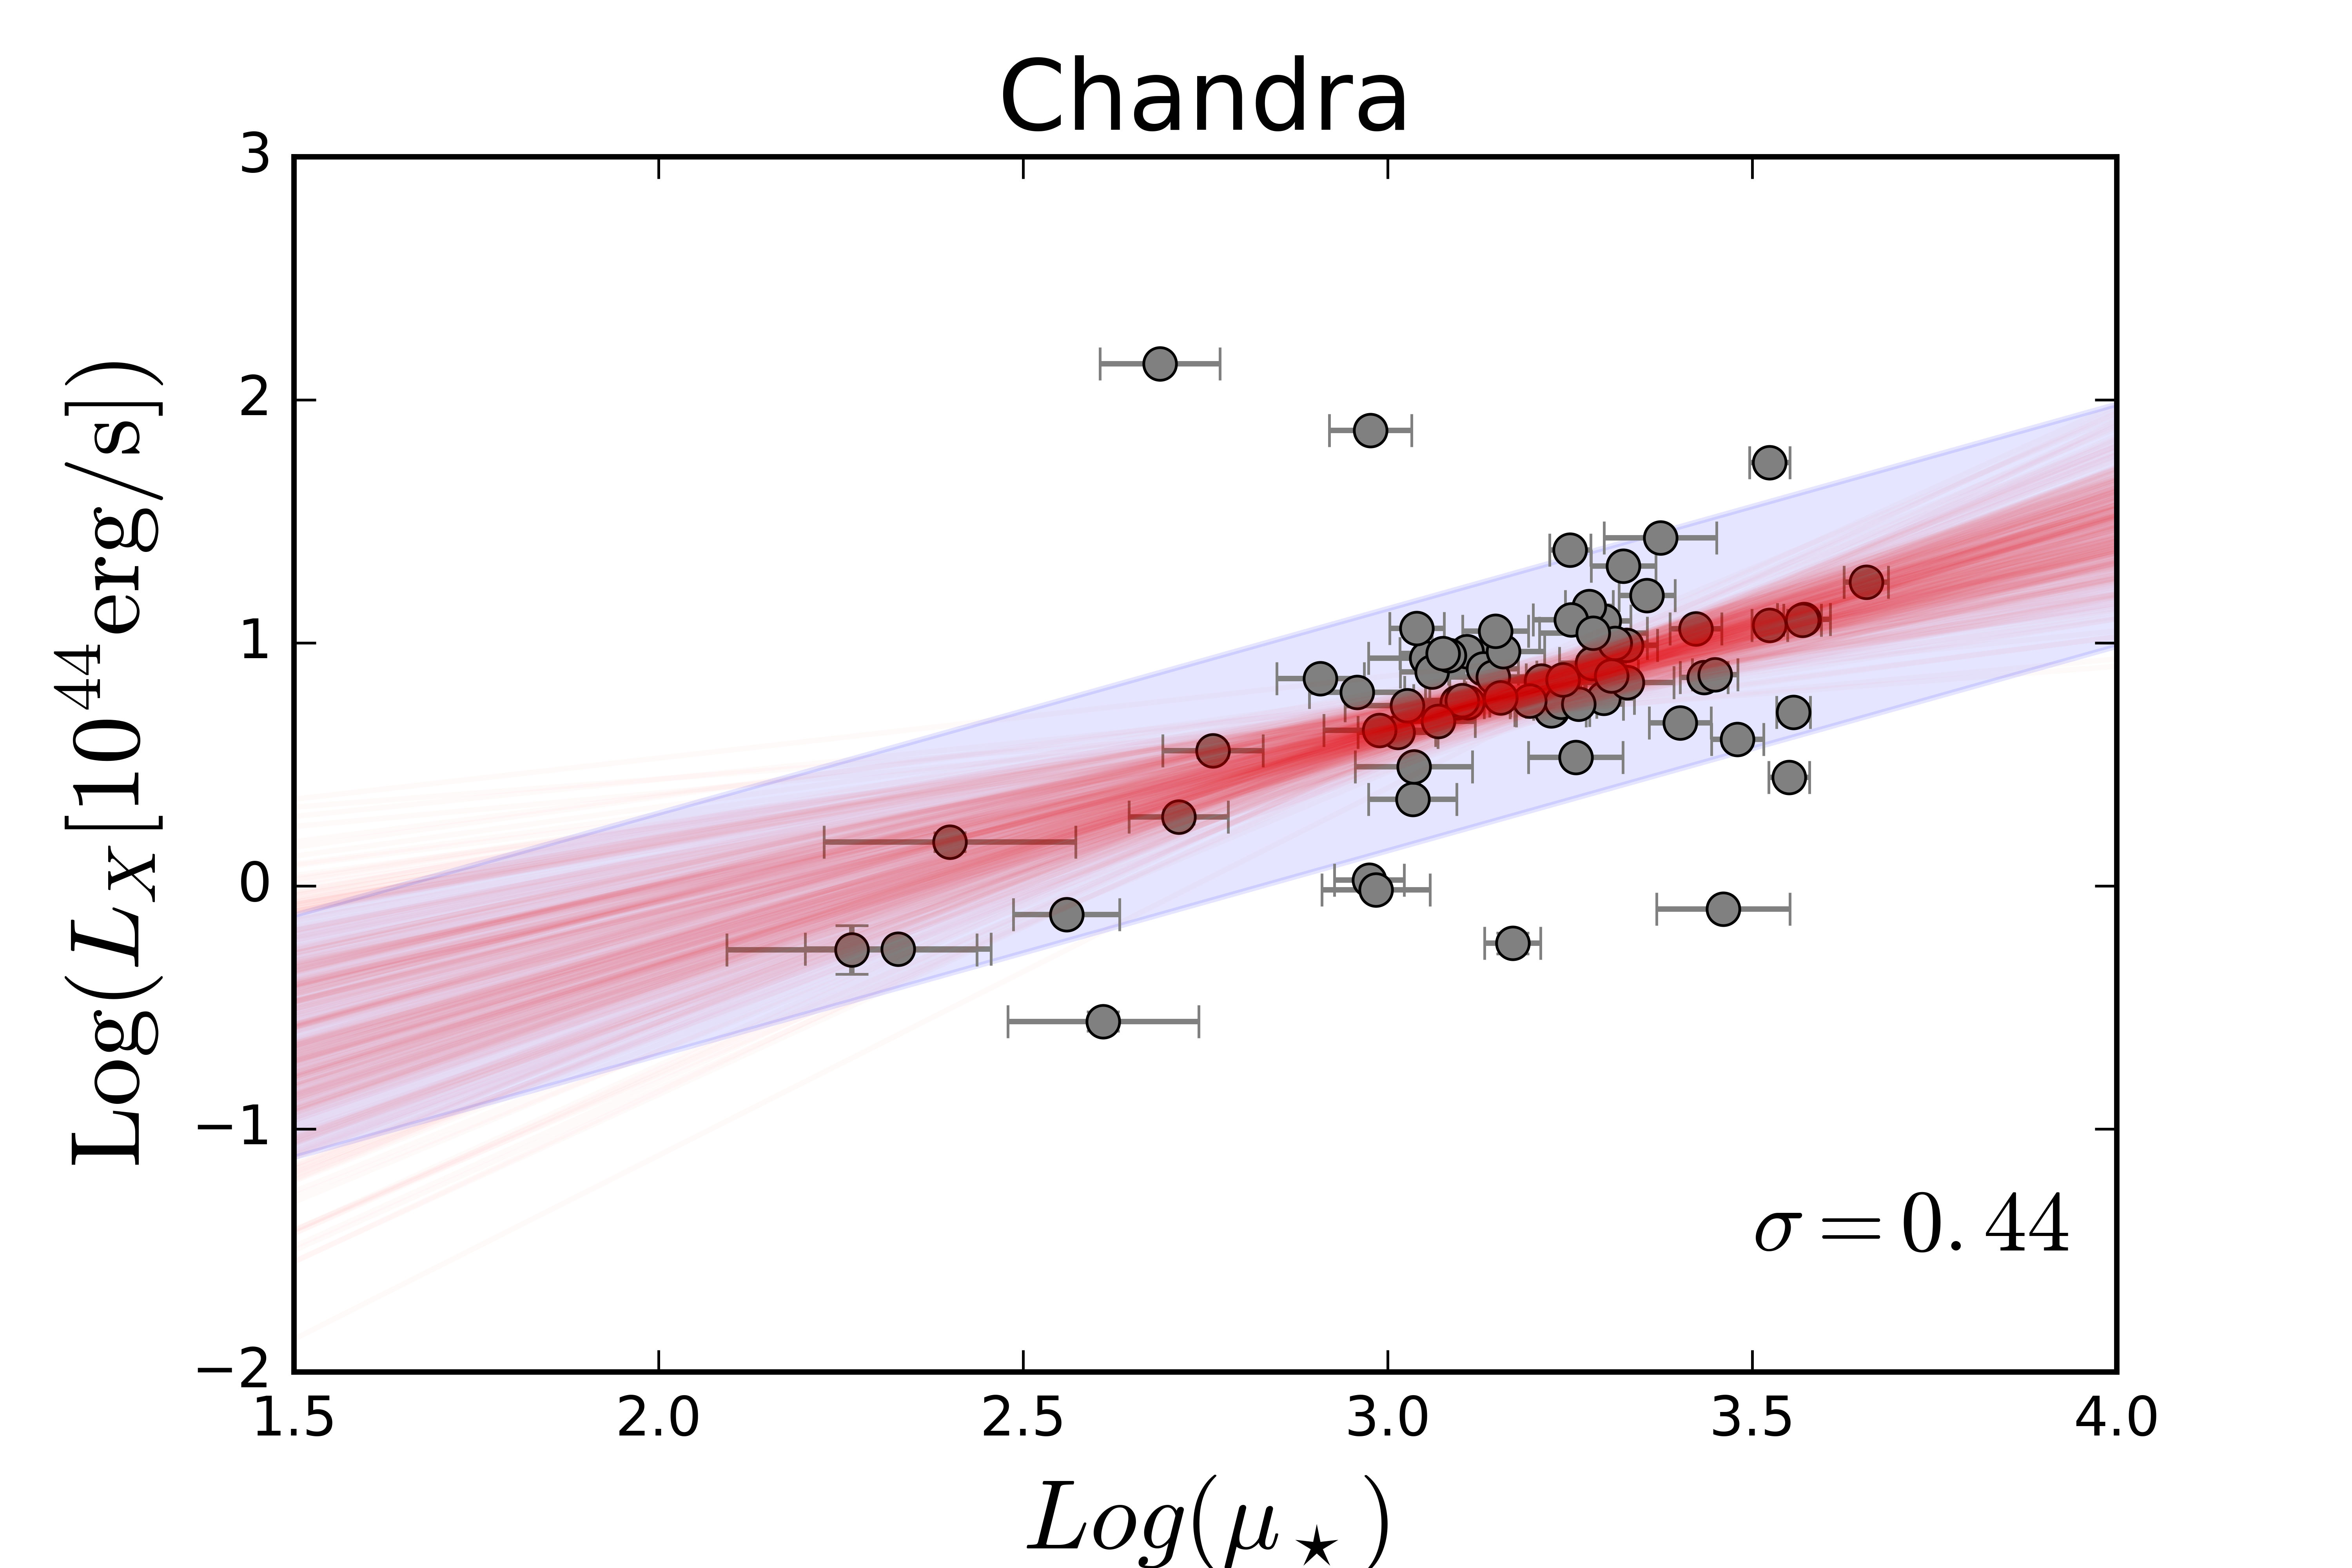
\includegraphics[width=0.7\textwidth]{./chapters/chapter5/figs/chandra_lx_mu_scatter_Feb18.png}\caption{Bayesian linear regression of $X$-ray luminosity and $\mu_\star$ for the XCS high signal-to-noise sample (top panel) and the Chandra sample (bottom panel). The grey points are our sample data points. The red lines are a random sample from the posterior distribution of slope and intercept, and the blue band represents 1$\sigma$ around the mean value of the intercept plus the intrinsic scatter.}\label{fig:lx}
\end{figure}

\subsection{Intrinsic scatter}

We find an intrinsic scatter of $\sigma_{{\rm Log} T_X|\mu_\star} = 0.152^{+0.017}_{-0.015}$ for the \emph{XMM} sample, which is only $\sim 2 \sigma$ above the value that we get if we reproduce the same analysis with the redMaPPer richness: $\sigma_{{\rm Log} T_X|\lambda} = 0.121^{+0.014}_{-0.013}$. This is a promising result in light of the fact that the redMapper mass proxy has been refined and optimised over several works (\citealt{lambda}, \citealt{rozo09}) and that the sample was selected using richness cuts ($\sigma_\lambda<15\%$, $\lambda>5$). No cuts have been performed based on $\mu_\star$.
The scatter on $T_X$ from the \emph{Chandra} sample is similar ($\sigma_{{\rm Log} T_X|\lambda} = 0.139^{+0.015}_{-0.014}$) and it is also less than $2\sigma$ above the redMaPPer richness estimate ($0.118^{+0.014}_{-0.014}$).

The value found for the \emph{XMM} scatter corresponds to a $41\%$ scatter (from $10^{\sigma}-1$): even though it is not straightforward to compare results computed with different methods and using different samples, several works find that the intrinsic scatter is $\sigma_{{\rm log} M_h|X} = 10-70\%$ for a mass proxy $X$ (see Table 3 of \citealt{mulroy} for a comparison). This result shows that our mass proxy is competitive with other methods of cluster mass estimation. Note that the scatter computed here is different from what we would find for the total cluster mass at fixed $\mu_\star$. In fact, as suggested in the previous subsection, not only do current X-ray temperature measurements probe a restricted cluster scale, but they are also influenced by gas and baryon physics. In other words, there is a non-negligible intrinsic scatter between total cluster mass and X-ray mass observables ($\sigma_{{\rm Log} L_X|M_h} \sim 0.17$ in \citealt{vikhlinin}).

We perform a number of tests to understand if the membership probabilities are taken into account in an optimal way. We find that including the blue cloud galaxies does not bring a significant increase in the scatter: the inclusion of the second term in the right-hand side of Eq. (\ref{eq:pc}), compared to having the red sequence term only or redMaPPer members only, brings an additional scatter which is an order of magnitude lower than the error. This is consistent with what we would expect for this sample, as it has been matched to a red-sequence cluster finder. \citet{extrinsicscatter} found that the blue galaxies significantly increase the scatter of their sample, but the fact that this is not true in our case allows us to keep this contribution which may become relevant at low richness and high redshift regimes, which should be tested using a non-red sequence based cluster finder and matched against other mass observables. It is beyond the scope of this work to test this hypothesis. \citet{extrinsicscatter} also show that differences between the true and predicted scatter of the mass proxy--mass relation are irrelevant for a DES--like survey as long as these differences are about 5\% or less (i.e., $\Delta \sigma < 0.05$), which further supports our choice.%{\bf {[Consider this in each of the tests]}}

We find that the inclusion of the radial probability  works well in terms of the choice of an arbitrary radial cut between $0.7$ and $3 h^{-1}$ Mpc: in fact, the intrinsic scatter of the temperature-mass relation is independent of this choice. On the other hand, we tested the use of the red galaxies only without including the radial probability contribution. In this case, we find similar trends to previous work (e.g. \citealt{andreon}): optimal choices for the aperture {\em do} exist when no membership probability is considered. We find that the scatter can increase by up to $\sim 15\%$ within the inner 1.5 Mpc, and outside that range mostly noise is added.

We tested the inclusion of color probabilities $p_c$ in the full membership probabilities by modifying Eq. (\ref{eq:pmem}) into $p_{\rm mem} = p_R p_z p_c$. We also tried to combine the color membership probabilities from different colors in different redshift ranges. This is justified by the fact that most of the colour information in a galaxy SED is contained in the 4000 \AA~ break, that shifts between the bands with redshift. We therefore use $g-r$ for the range $z<0.35$, $r-i$ in $0.35<z<0.75$ and $i-z$ at $z>0.75$. We find that these tests did not have a significant impact on the mean scaling relation fit and intrinsic scatter, so it is reasonable to include the simpler version of the full probabilities as given in Eq. (\ref{eq:pmem}).

The fact that our scaling relation scatter and slope are insensitive to the choices made in these tests shows that the membership probabilities are robust and that cluster size and colors (that enter in $p_{\rm mem}$ though the redshift probability estimation) are taken into account well.

Finally, we estimate the scatter of halo mass at fixed mass proxy, which is a quantity of interest in cosmological studies. In fact, the halo mass scatter about the mean mass--observable relation is one of the main systematics that need to be taken into account. We follow \citet{2014ApJ...783...80R} and estimate this quantity through:
\begin{equation}
\sigma^2_{M|\mu_\star} = \frac{\sigma^2_{T_X|\mu_\star}}{\beta^2_{M|T_X}}-\sigma^2_{M|T_X}\, , \label{eq:sigmaM}
\end{equation}
where variables are in natural logarithm (in order to use results from the literature), the scatter in mass at fixed $T_X$ has a fiducial value of 15\% and the slope of the $M-T_X$ relation is $\beta=1.5$. We find that $\sigma_{{\rm Log}M|{\rm Log}\mu_\star} \sim 0.19$, while $\sigma_{{\rm Log}M|{\rm Log}\lambda} \sim 0.12$ for the XMM sample. \citet{2014ApJ...783...80R} also find $\sigma_{{\rm Log}M|{\rm Log}\lambda} \sim 0.11$ when comparing redMaPPer SDSS measurements to \emph{XCS} temperatures. Note that this is only a qualitative estimate of the scatter on halo mass, and the results presented are only used to investigate the performance of our mass proxy. A careful modeling of the cluster selection effects, an estimate of the correlation coefficient for $\mu_\star-T_X$ to be included in Eq. (\ref{eq:sigmaM}), simulations and Fisher matrix forecasts would be needed in order to evaluate the actual impact of $\mu_\star$ on cosmological parameters. DES collaborators Farahi et al., in prep., are already working on a similar modeling for $\lambda$. Based on their results, the error on the scatter on halo mass at fixed richness is large enough to make $\sigma_{{\rm Log}M|{\rm Log}\lambda}$ and $\sigma_{{\rm Log}M|{\rm Log}\mu_\star}$ consistent within $1\sigma$. In the future, we plan on studying these effects for $\mu_\star$ as well.

\section{Weak lensing calibration}\label{wlcalib}


\begin{figure}
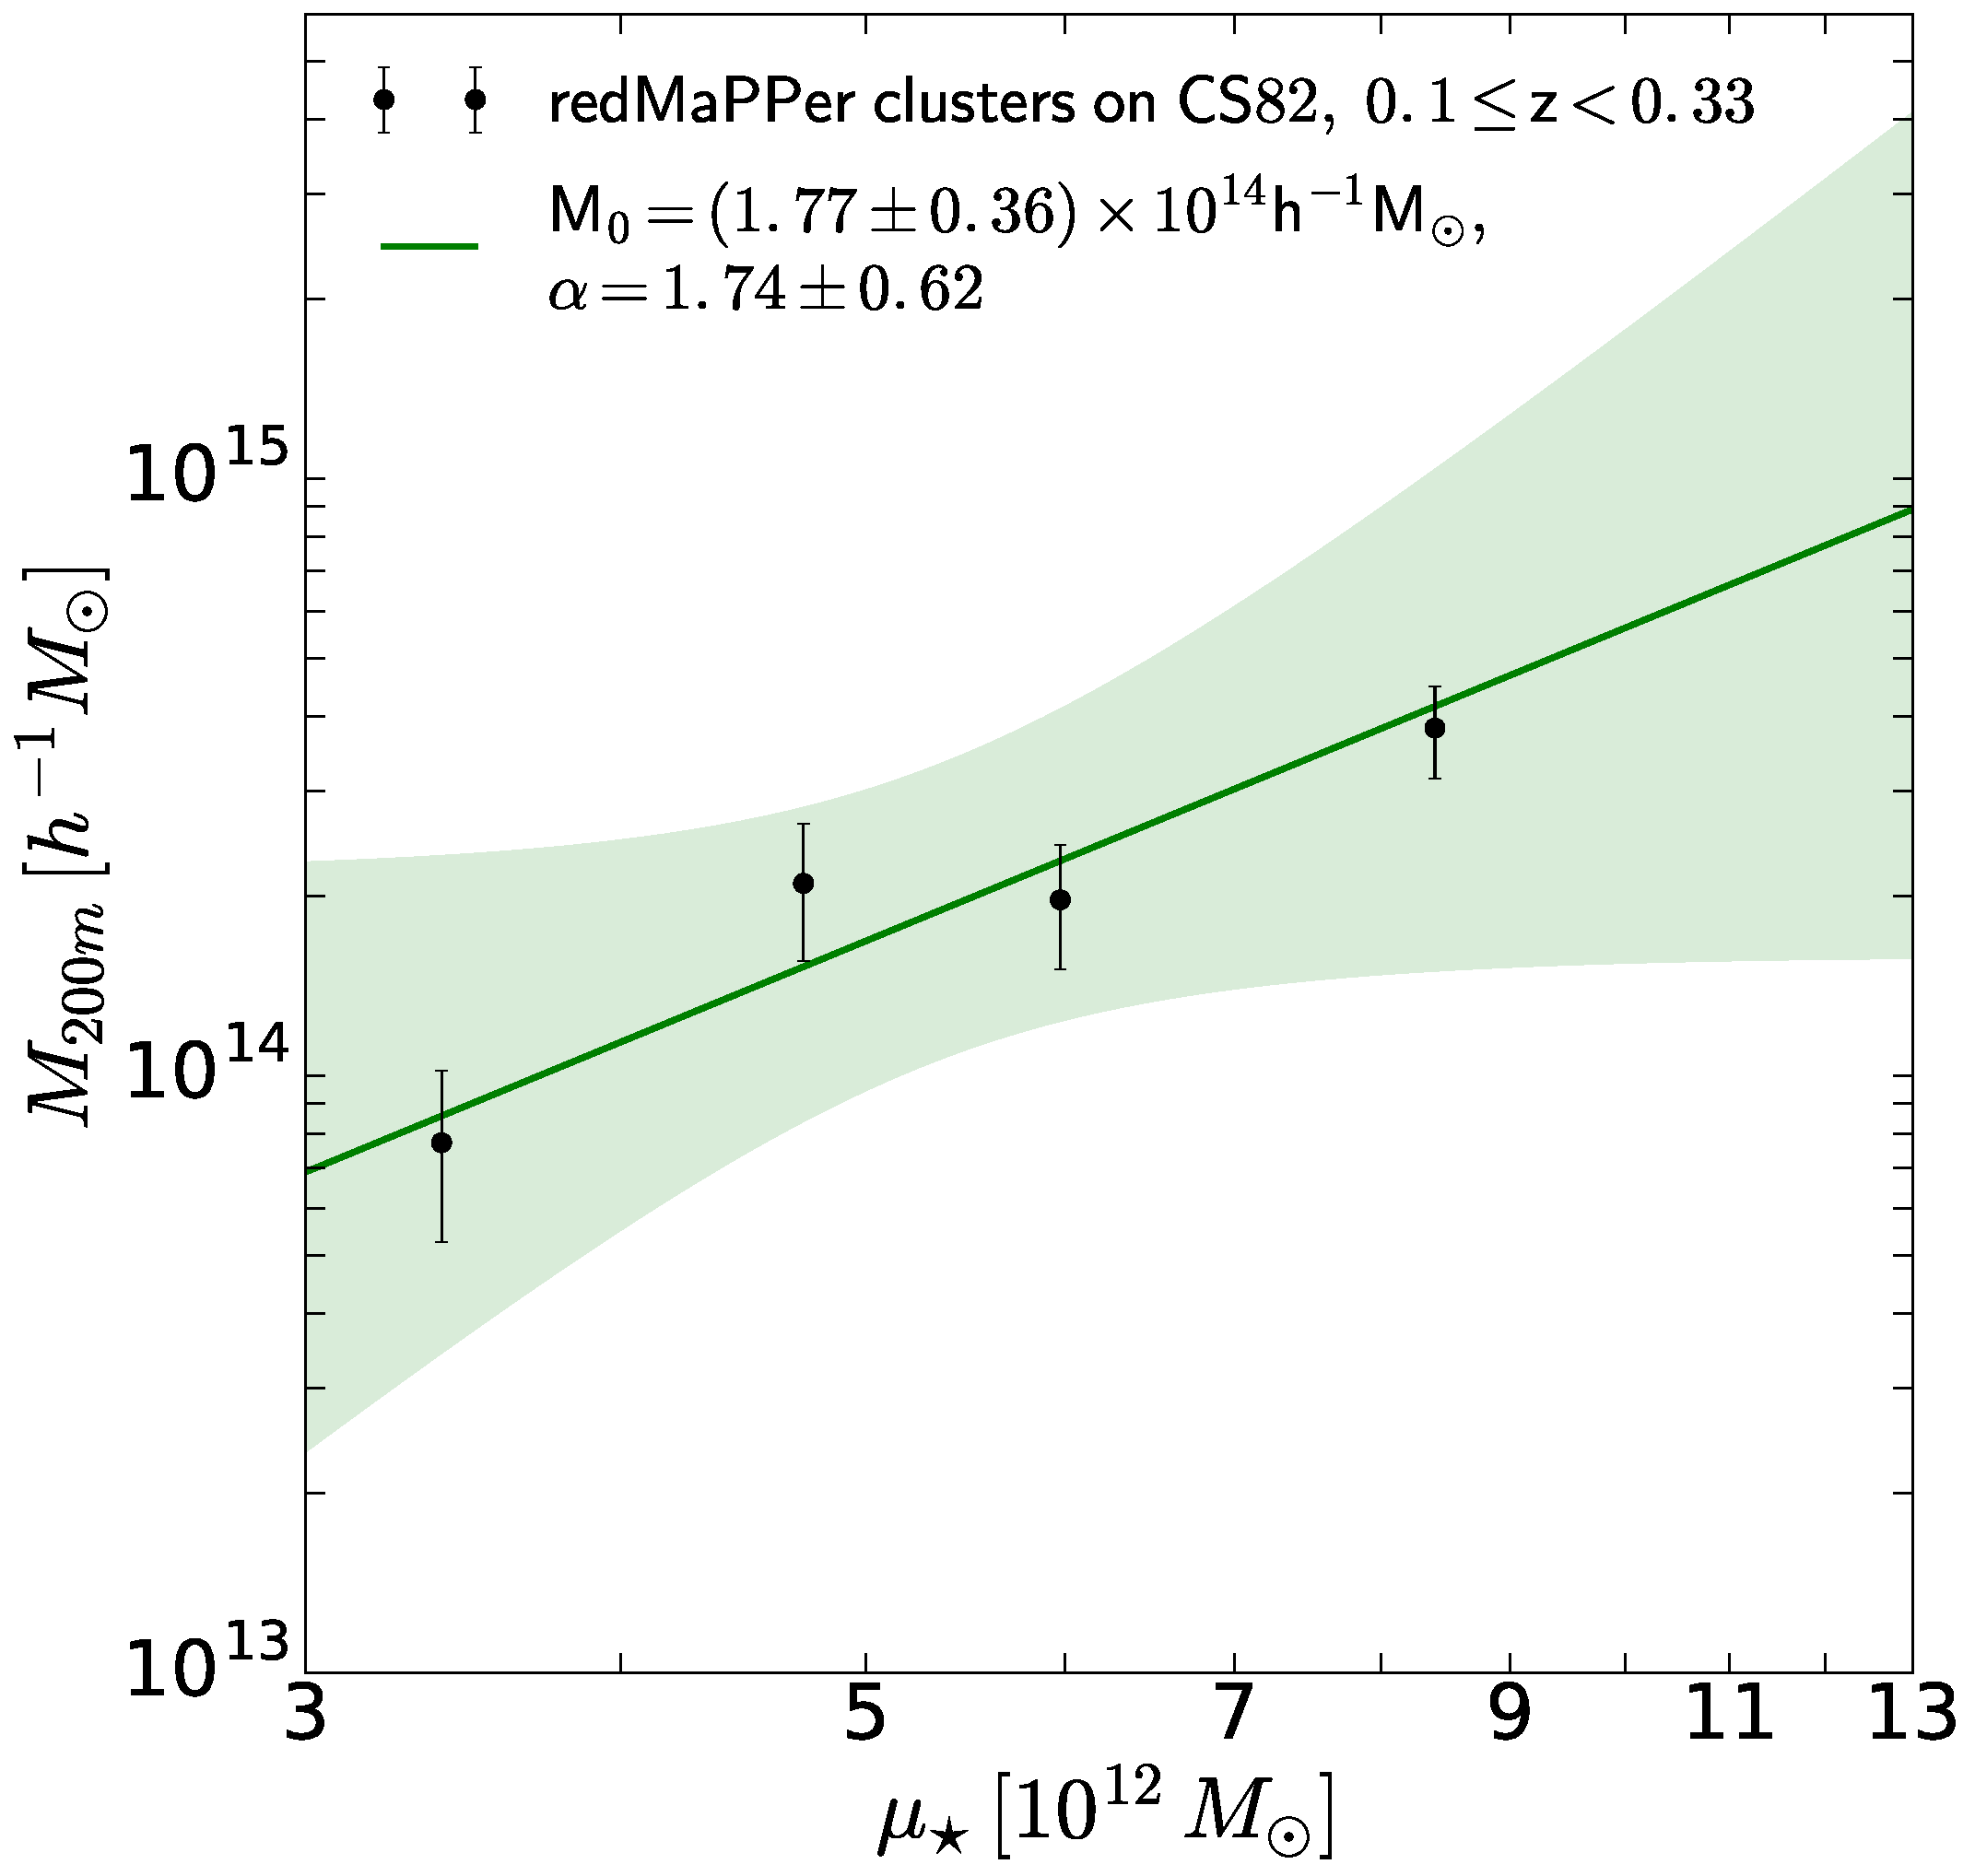
\includegraphics[width=0.33\textwidth]{./chapters/chapter5/figs/mass_richness_lowz_mustar_MEpivotMedianMiscV2.pdf}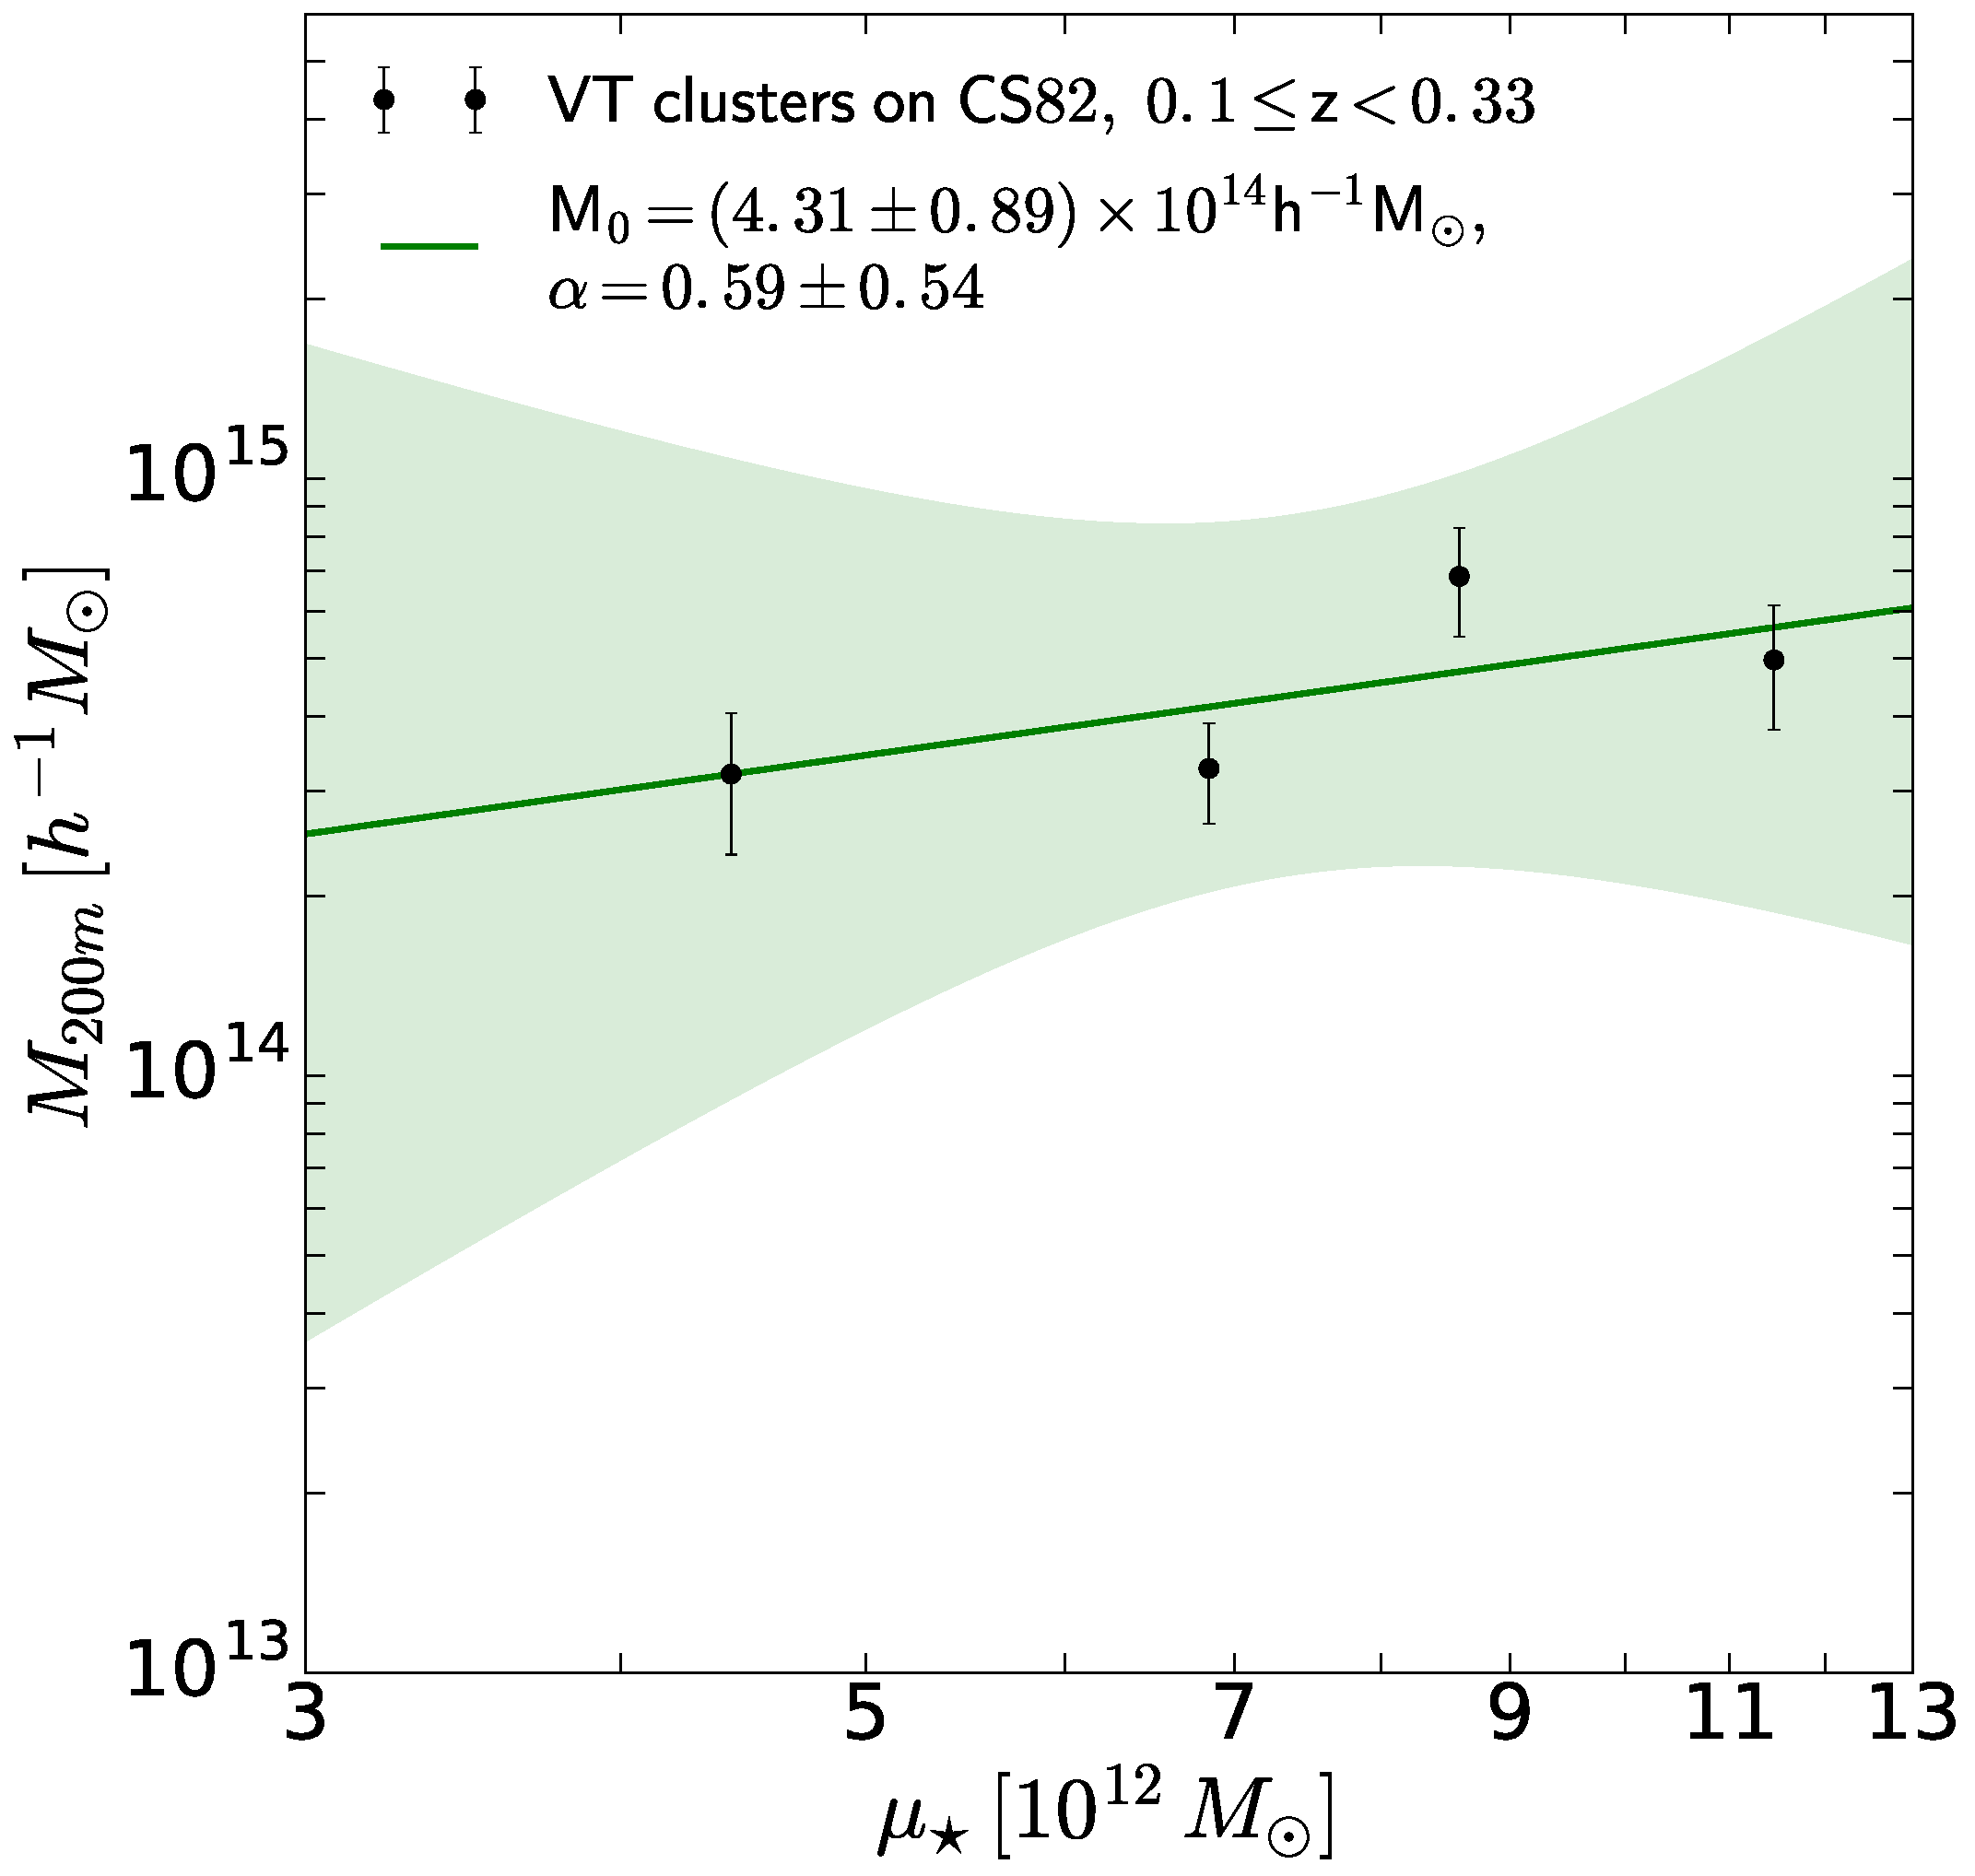
\includegraphics[width=0.33\textwidth]{./chapters/chapter5/figs/mass_richness_VT_lowz_mustar_MEpivotMedianMiscV2.pdf}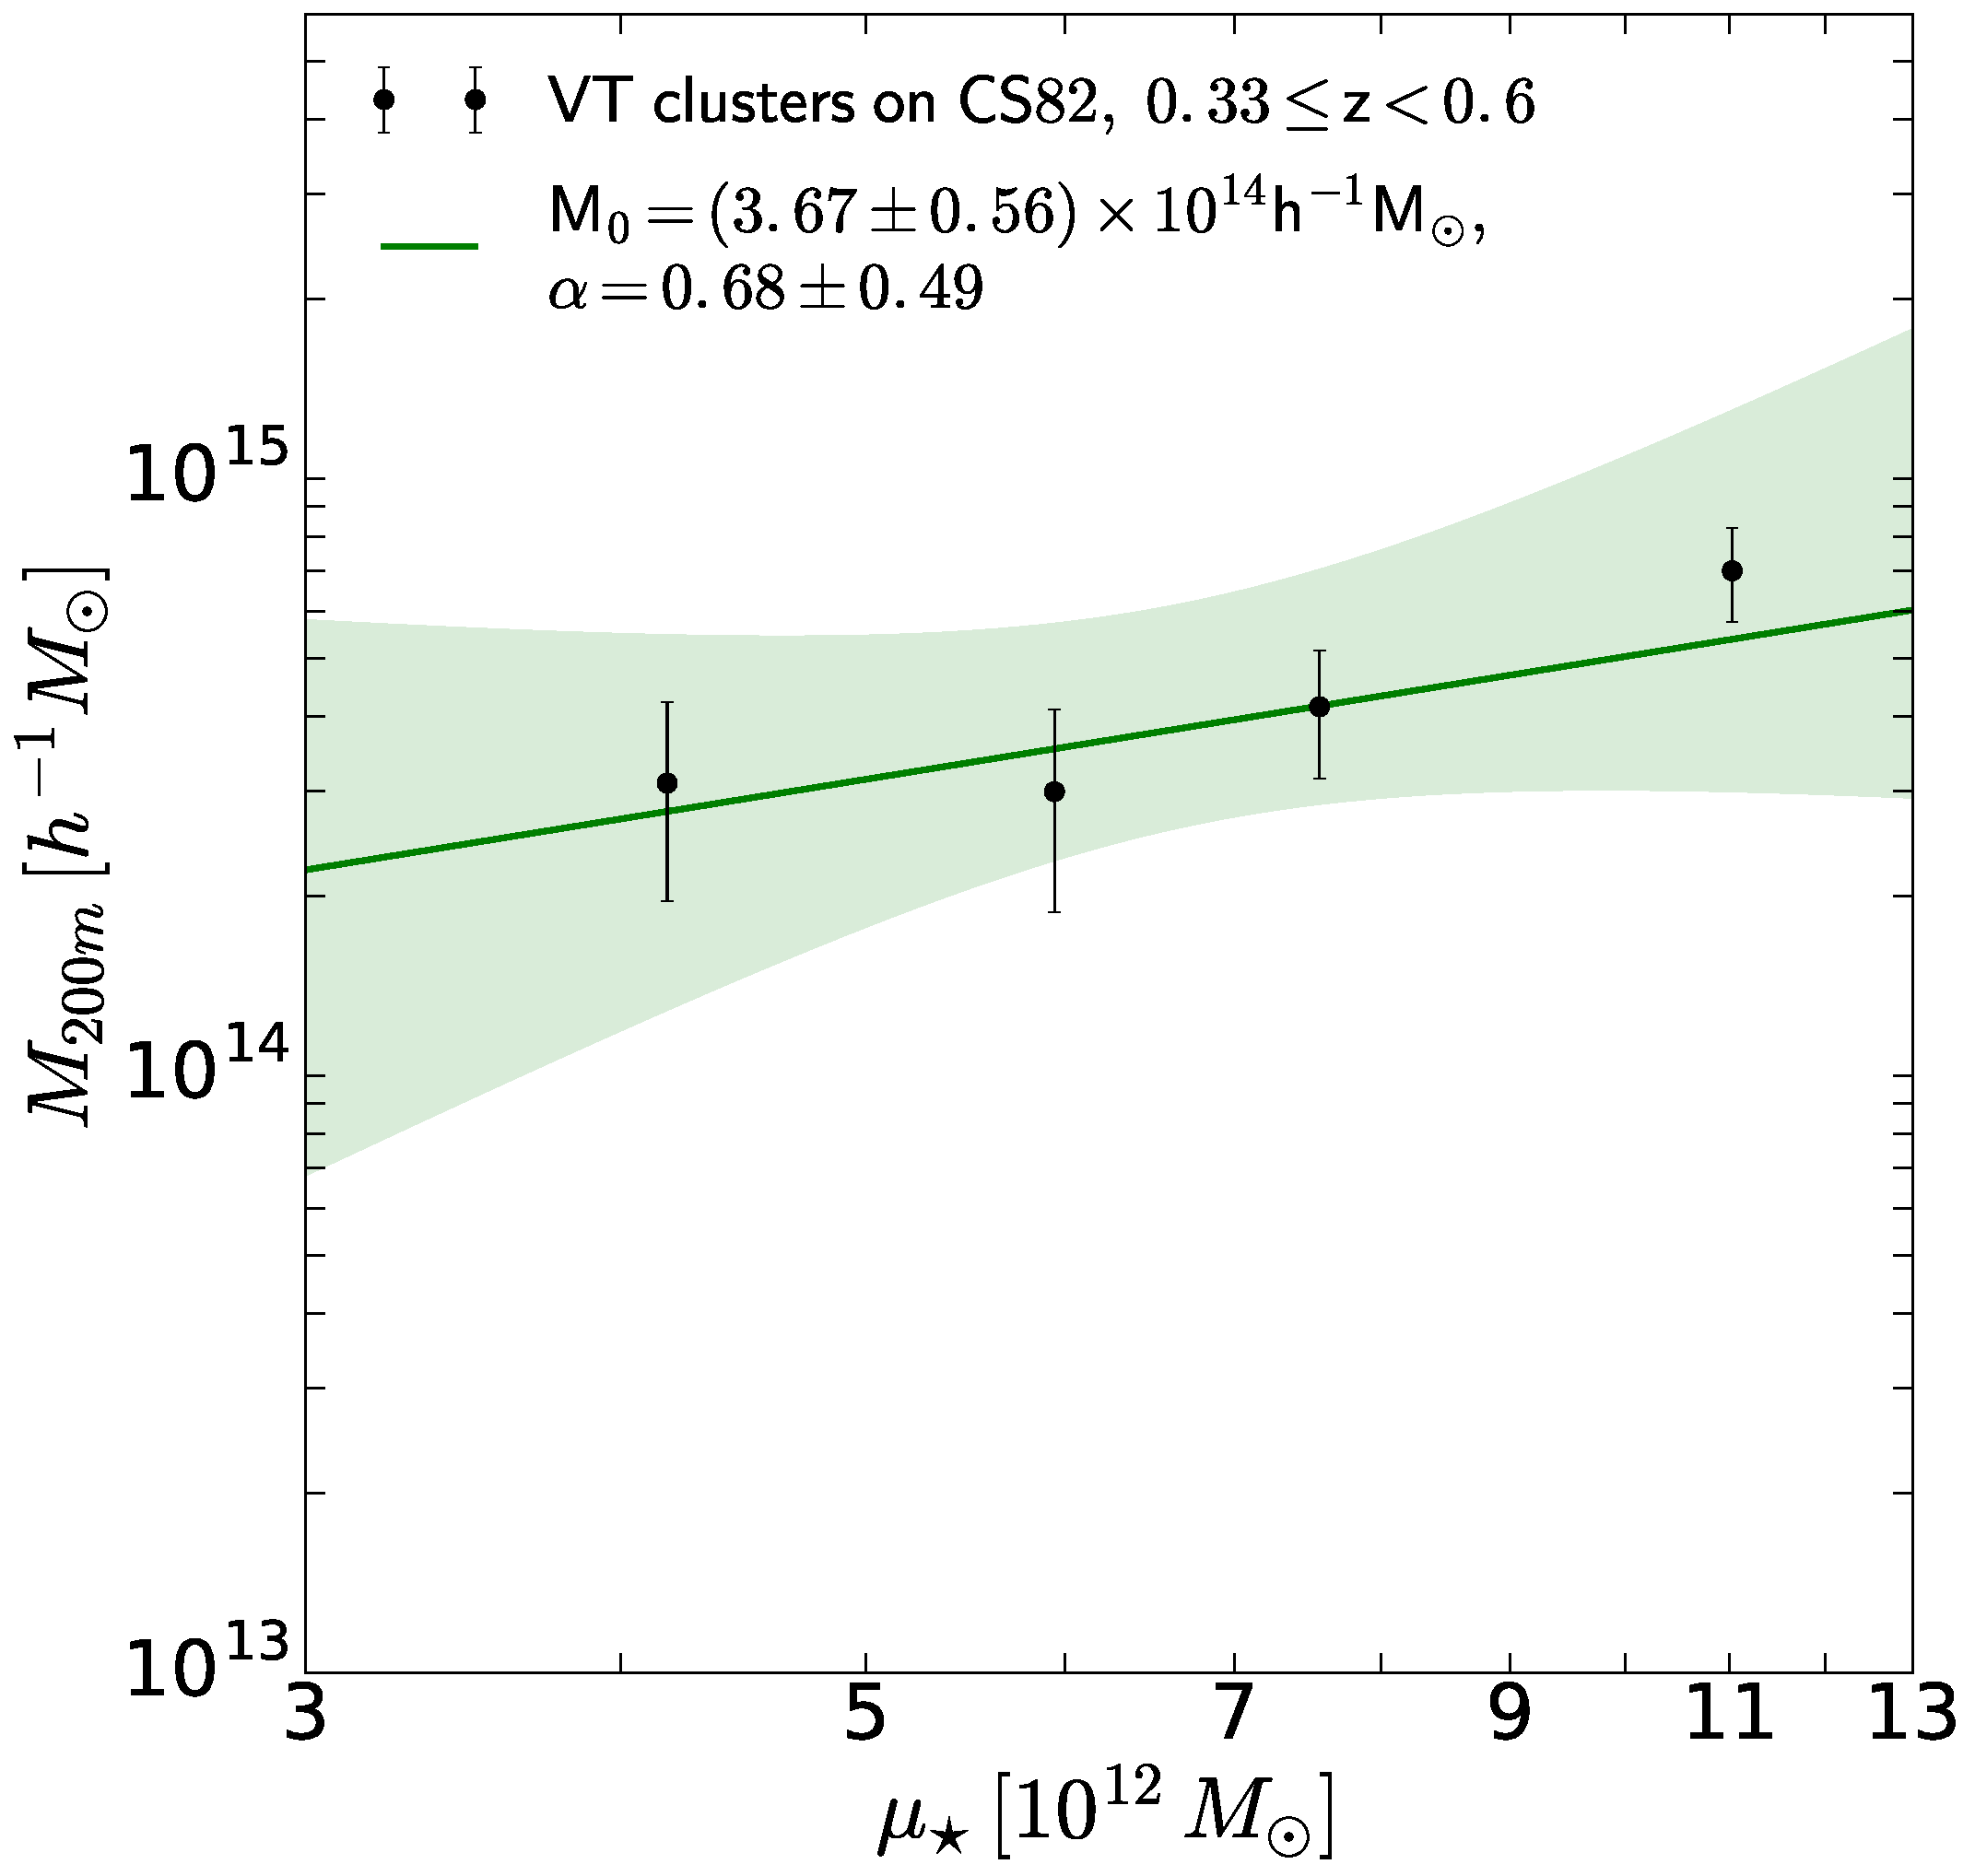
\includegraphics[width=0.33\textwidth]{./chapters/chapter5/figs/mass_richness_VT_midz_mustar_MEpivotMedianMiscV2.pdf}\caption{Weak lensing mass calibration of $\mu_\star$ from \citet{maria}. The shaded regions represent $2\sigma$ confidence intervals. Miscentering corrections have been applied to the mass estimates. In the mass--$\mu_{\star}$ relation we adopt the median of $\mu_{\star}$ as the mass proxy pivot, which is, in order for the three panels: $\mu_{\star}^0 = 5.16 \times 10^{12} M_{\odot}$ (redMaPPer low redshift sample), $\mu_{\star}^0 = 7.30 \times 10^{12} M_{\odot}$ (VT low redshift sample), $\mu_{\star}^0 = 6.30 \times 10^{12} M_{\odot}$(VT high redshift sample). In this work, we decided to leave $\mu_\star$ in units of $M_\odot$, so the factor $10^{-10} M_\odot^{-1}$ from Eq. (\ref{eq:mustar}) is not taken into account.}\label{fig:wlcalib}
\end{figure}

In \citet{maria} we use two cluster samples from the SDSS Stripe 82 data to calibrate $\mu_\star$ and $\lambda$ against weak lensing measurements: 230 redMaPPer clusters at redshift $0.1\leq z<0.33$ and 136 VT clusters at $0.1 \leq z < 0.6$. The source galaxy catalog used comes from the CS82 survey \citep{erben2017}, with shape measurements and photometric redshifts from matched SDSS co-add \citep{2014ApJ...794..120A} and UKIDSS YJHK \citep{UKIDSS} photometry. Clusters are stacked in $\mu_{\star}$ bins to measure a mass-observable power law relation of the form:
\begin{equation}
\langle M_{200c} | \mu_{\star} \rangle = M_0 \left(\frac{\mu_{\star}}{\mu_{\star}^0}\right)^{\alpha}\,.
\label{massstellar}
\end{equation}
Mass proxy bins have been chosen in order to have a similar number of clusters in each bin. For redMaPPer clusters we obtain $M_0 = (1.77 \pm 0.36) \times 10^{14}h^{-1} M_{\odot}$, $\alpha = 1.74 \pm 0.62$, while for VT clusters: $M_0 = (4.31 \pm 0.89) \times 10^{14}h^{-1} M_{\odot}$, $\alpha = 0.59 \pm 0.54$ and $M_0 = (3.67 \pm 0.56) \times 10^{14}h^{-1} M_{\odot}$, $\alpha = 0.68 \pm 0.49$ for the low and high redshift bins, respectively. This fits are shown in Figure \ref{fig:wlcalib}. The results found for the redMaPPer richness with this method ($M_0 = (2.46 \pm 0.44) \times 10^{14}h^{-1} M_{\odot}$, $\alpha = 1.18 \pm 0.38$) are consistent with the literature (\citealt{2017MNRAS.466.3103S,2017MNRAS.469.4899M,oguri}), showing that this method can be applied to any cluster-finding algorithm, including VT. The on--going work consists in replicating this analysis using DES Year 3 data, which comprises of a larger and deeper sample than SDSS.




\section{Conclusions}\label{sec:conclusion}
%%{\bf {[To provide a quantitative estimate of the impact of the scatter on the FoM can find/ask for the Fisher forecasting code of Wu et al. (2010) or Wu, Rozo \& Welscher 2008 as done in Mantz et al. 2017. ]}}
%%Could do as in the Fahari et al in prep paper for X ray sample and get the scatter on total mass from X ray??
In this Chapter we presented a stellar mass based mass proxy that can be applied to photometric surveys. Our main results can be summarised as follows:

\begin{itemize}
\item The outputs of our BMA code presented in Chapter 2 are used to estimate our mass proxy $\mu_\star$ for DES Year 1 data. We study the scatter of this mass proxy compared to X-ray mass observables: we find $\sigma_{{\rm Log}T_X|\mu_\star}=0.152^{+0.017}_{-0.015}$ and $0.138^{+0.015}_{-0.014}$ for the \emph{XMM} and \emph{Chandra} temperatures respectively. These values are consistent within $2\sigma$ with the results from the redMaPPer richness $\lambda$. Given that $\lambda$ has been extensively studied and optimised to reach the lowest levels in scatter, we conclude that also $\mu_\star$ is a promising low--scatter mass proxy.

%less than 2$\sigma$ above the scatter we measure with the widely used redMaPPer richness $\lambda$. This measurement shows that $\mu_\star$ is a promising low--scatter mass proxy.

\item It is a sensible choice to develop a new mass proxy using a well known sample of clusters, and also to compare results with a well--established mass proxy in order to validate the method used. In this spirit, $\mu_\star$ has been calibrated with weak lensing measurements for redMaPPer and VT clusters from SDSS and CS82 data. The analysis has been performed also with the redMaPPer richness, where results are consistent with others from the literature, showing that it is robust. The slope found in the mass proxy--halo mass relation for redMaPPer clusters is similar for $\lambda$ and $\mu_\star$. This indicates that the correlation of our mass proxy with halo mass is just as good as for the redMaPPer proxy. However, this comparison is only valid where $\lambda$ is available, i.e. in SDSS clusters which only go out to redshift 0.3. It is in our interests to explore comparisons with red--sequence cluster finder out to larger redshifts, where the red sequence width increases. The same analysis is currently being performed for DES Year 3 data, where clusters are probed out to $z\lesssim1$.

\item Future work will include the development of a new version of the VT cluster finder, that integrates this mass proxy into the pipeline (Bugard et al., in prep.), and a production of a cluster catalog for DES data. We also plan to perform an ``end--to--end'' analysis to quantify the impact of this mass proxy on cosmological parameters.  

\end{itemize}



